%%%%%%%%%%%%%%%%%%%%%%%%%%%%%%%%%%%%%%%%%
% Cleese Assignment (For Students)
% LaTeX Template
% Version 2.0 (27/5/2018)
%
% This template originates from:
% http://www.LaTeXTemplates.com
%
% Author:
% Vel (vel@LaTeXTemplates.com)
%
% License:
% CC BY-NC-SA 3.0 (http://creativecommons.org/licenses/by-nc-sa/3.0/)
% 
%%%%%%%%%%%%%%%%%%%%%%%%%%%%%%%%%%%%%%%%%

%----------------------------------------------------------------------------------------
%	PACKAGES AND OTHER DOCUMENT CONFIGURATIONS
%----------------------------------------------------------------------------------------

\documentclass[11pt]{article}
\usepackage{float}

%\usepackage[printwatermark]{xwatermark}
%\newwatermark[allpages,color=gray!50,angle=45,scale=2.5,xpos=-5,ypos=-5]{Mohammad Hadi}

%%%%%%%%%%%%%%%%%%%%%%%%%%%%%%%%%%%%%%%%%
% Cleese Assignment
% Structure Specification File
% Version 1.0 (27/5/2018)
%
% This template originates from:
% http://www.LaTeXTemplates.com
%
% Author:
% Vel (vel@LaTeXTemplates.com)
%
% License:
% CC BY-NC-SA 3.0 (http://creativecommons.org/licenses/by-nc-sa/3.0/)
% 
%%%%%%%%%%%%%%%%%%%%%%%%%%%%%%%%%%%%%%%%%

%----------------------------------------------------------------------------------------
%	PACKAGES AND OTHER DOCUMENT CONFIGURATIONS
%----------------------------------------------------------------------------------------

\usepackage{lastpage} % Required to determine the last page number for the footer

\usepackage{graphicx} % Required to insert images

\setlength\parindent{0pt} % Removes all indentation from paragraphs

\usepackage[most]{tcolorbox} % Required for boxes that split across pages

\usepackage{booktabs} % Required for better horizontal rules in tables

\usepackage{listings} % Required for insertion of code

\usepackage{etoolbox} % Required for if statements

%----------------------------------------------------------------------------------------
%	MARGINS
%----------------------------------------------------------------------------------------

\usepackage{geometry} % Required for adjusting page dimensions and margins

\geometry{
	paper=a4paper, % Change to letterpaper for US letter
	top=3cm, % Top margin
	bottom=3cm, % Bottom margin
	left=2.5cm, % Left margin
	right=2.5cm, % Right margin
	headheight=14pt, % Header height
	footskip=1.4cm, % Space from the bottom margin to the baseline of the footer
	headsep=1.2cm, % Space from the top margin to the baseline of the header
	%showframe, % Uncomment to show how the type block is set on the page
}

%----------------------------------------------------------------------------------------
%	FONT
%----------------------------------------------------------------------------------------

\usepackage[utf8]{inputenc} % Required for inputting international characters
\usepackage[T1]{fontenc} % Output font encoding for international characters

\usepackage[sfdefault,light]{roboto} % Use the Roboto font

%----------------------------------------------------------------------------------------
%	HEADERS AND FOOTERS
%----------------------------------------------------------------------------------------

\usepackage{fancyhdr} % Required for customising headers and footers

\pagestyle{fancy} % Enable custom headers and footers

\lhead{\small\assignmentClass\ifdef{\assignmentClassInstructor}{\ (\assignmentClassInstructor):}{}\ \assignmentTitle} % Left header; output the instructor in brackets if one was set
\chead{} % Centre header
\rhead{\small\ifdef{\assignmentAuthorName}{\assignmentAuthorName}{\ifdef{\assignmentDueDate}{Due\ \assignmentDueDate}{}}} % Right header; output the author name if one was set, otherwise the due date if that was set

\lfoot{} % Left footer
\cfoot{\small Page\ \thepage\ of\ \pageref{LastPage}} % Centre footer
\rfoot{} % Right footer

\renewcommand\headrulewidth{0.5pt} % Thickness of the header rule

%----------------------------------------------------------------------------------------
%	MODIFY SECTION STYLES
%----------------------------------------------------------------------------------------

\usepackage{titlesec} % Required for modifying sections

%------------------------------------------------
% Section

\titleformat
{\section} % Section type being modified
[block] % Shape type, can be: hang, block, display, runin, leftmargin, rightmargin, drop, wrap, frame
{\Large\bfseries} % Format of the whole section
{\assignmentQuestionName~\thesection} % Format of the section label
{6pt} % Space between the title and label
{} % Code before the label

\titlespacing{\section}{0pt}{0.5\baselineskip}{0.5\baselineskip} % Spacing around section titles, the order is: left, before and after

%------------------------------------------------
% Subsection

\titleformat
{\subsection} % Section type being modified
[block] % Shape type, can be: hang, block, display, runin, leftmargin, rightmargin, drop, wrap, frame
{\itshape} % Format of the whole section
{(\alph{subsection})} % Format of the section label
{4pt} % Space between the title and label
{} % Code before the label

\titlespacing{\subsection}{0pt}{0.5\baselineskip}{0.5\baselineskip} % Spacing around section titles, the order is: left, before and after

\renewcommand\thesubsection{(\alph{subsection})}

%----------------------------------------------------------------------------------------
%	CUSTOM QUESTION COMMANDS/ENVIRONMENTS
%----------------------------------------------------------------------------------------

% Environment to be used for each question in the assignment
\newenvironment{question}{
	\vspace{0.5\baselineskip} % Whitespace before the question
	\section{} % Blank section title (e.g. just Question 2)
	\lfoot{\small\itshape\assignmentQuestionName~\thesection~continued on next page\ldots} % Set the left footer to state the question continues on the next page, this is reset to nothing if it doesn't (below)
}{
	\lfoot{} % Reset the left footer to nothing if the current question does not continue on the next page
}

%------------------------------------------------

% Environment for subquestions, takes 1 argument - the name of the section
\newenvironment{subquestion}[1]{
	\subsection{#1}
}{
}

%------------------------------------------------

% Command to print a question sentence
\newcommand{\questiontext}[1]{
	\textbf{#1}
	\vspace{0.5\baselineskip} % Whitespace afterwards
}

%------------------------------------------------

% Command to print a box that breaks across pages with the question answer
\newcommand{\answer}[1]{
	\begin{tcolorbox}[breakable, enhanced]
		#1
	\end{tcolorbox}
}

%------------------------------------------------

% Command to print a box that breaks across pages with the space for a student to answer
\newcommand{\answerbox}[1]{
	\begin{tcolorbox}[breakable, enhanced]
		\vphantom{L}\vspace{\numexpr #1-1\relax\baselineskip} % \vphantom{L} to provide a typesetting strut with a height for the line, \numexpr to subtract user input by 1 to make it 0-based as this command is
	\end{tcolorbox}
}

%------------------------------------------------

% Command to print an assignment section title to split an assignment into major parts
\newcommand{\assignmentSection}[1]{
	{
		\centering % Centre the section title
		\vspace{2\baselineskip} % Whitespace before the entire section title
		
		\rule{0.8\textwidth}{0.5pt} % Horizontal rule
		
		\vspace{0.75\baselineskip} % Whitespace before the section title
		{\LARGE \MakeUppercase{#1}} % Section title, forced to be uppercase
		
		\rule{0.8\textwidth}{0.5pt} % Horizontal rule
		
		\vspace{\baselineskip} % Whitespace after the entire section title
	}
}

%----------------------------------------------------------------------------------------
%	TITLE PAGE
%----------------------------------------------------------------------------------------

\author{\textbf{\assignmentAuthorName}} % Set the default title page author field
\date{} % Don't use the default title page date field

\title{
	\thispagestyle{empty} % Suppress headers and footers
	\vspace{0.2\textheight} % Whitespace before the title
	\textbf{\assignmentClass:\ \assignmentTitle}\\[-4pt]
	\ifdef{\assignmentDueDate}{{\small Due\ on\ \assignmentDueDate}\\}{} % If a due date is supplied, output it
	\ifdef{\assignmentClassInstructor}{{\large \textit{\assignmentClassInstructor}}}{} % If an instructor is supplied, output it
	\vspace{0.32\textheight} % Whitespace before the author name
}
 % Include the file specifying the document structure and custom commands

%----------------------------------------------------------------------------------------
%	ASSIGNMENT INFORMATION
%----------------------------------------------------------------------------------------

% Required
\newcommand{\assignmentQuestionName}{Experiment} % The word to be used as a prefix to question numbers; example alternatives: Problem, Exercise
\newcommand{\assignmentClass}{Electrical Circuits Lab (Taught by Mohammad Hadi)\\Manual 1 (Due on DDD.,\ mmm.\ dd,\ yyyy)} % Course (Lecturer)\\Assignment (Due date)
\newcommand{\assignmentTitle}{} % Assignment title or name
\newcommand{\assignmentAuthorName}{Sina Hashemi \& M.Mahdi Shokrzade\\402102668 - 402101985} % Student name\\Student number
%----------------------------------------------------------------------------------------

\newcommand{\PicScale}{0.25}

\begin{document}
\textbf{An oscilloscope is an electronic measuring device which provides a two-dimensional time-domain visual representation of electrical signals. In this experiment, you learn how to use a digital oscilloscope.
}
%----------------------------------------------------------------------------------------
%	TITLE PAGE
%----------------------------------------------------------------------------------------

\assignmentSection{Mandatory Experiments}

%----------------------------------------------------------------------------------------
%	QUESTION 1
%----------------------------------------------------------------------------------------


\begin{question}

    \questiontext{Download the catalog of the lab oscilloscope. Review the catalog and describe the functionality of the major control groups on the oscilloscope including  display group, vertical group, horizontal group, and trigger group.}

    \answer{
        \begin{figure}[H]
            \begin{center}
                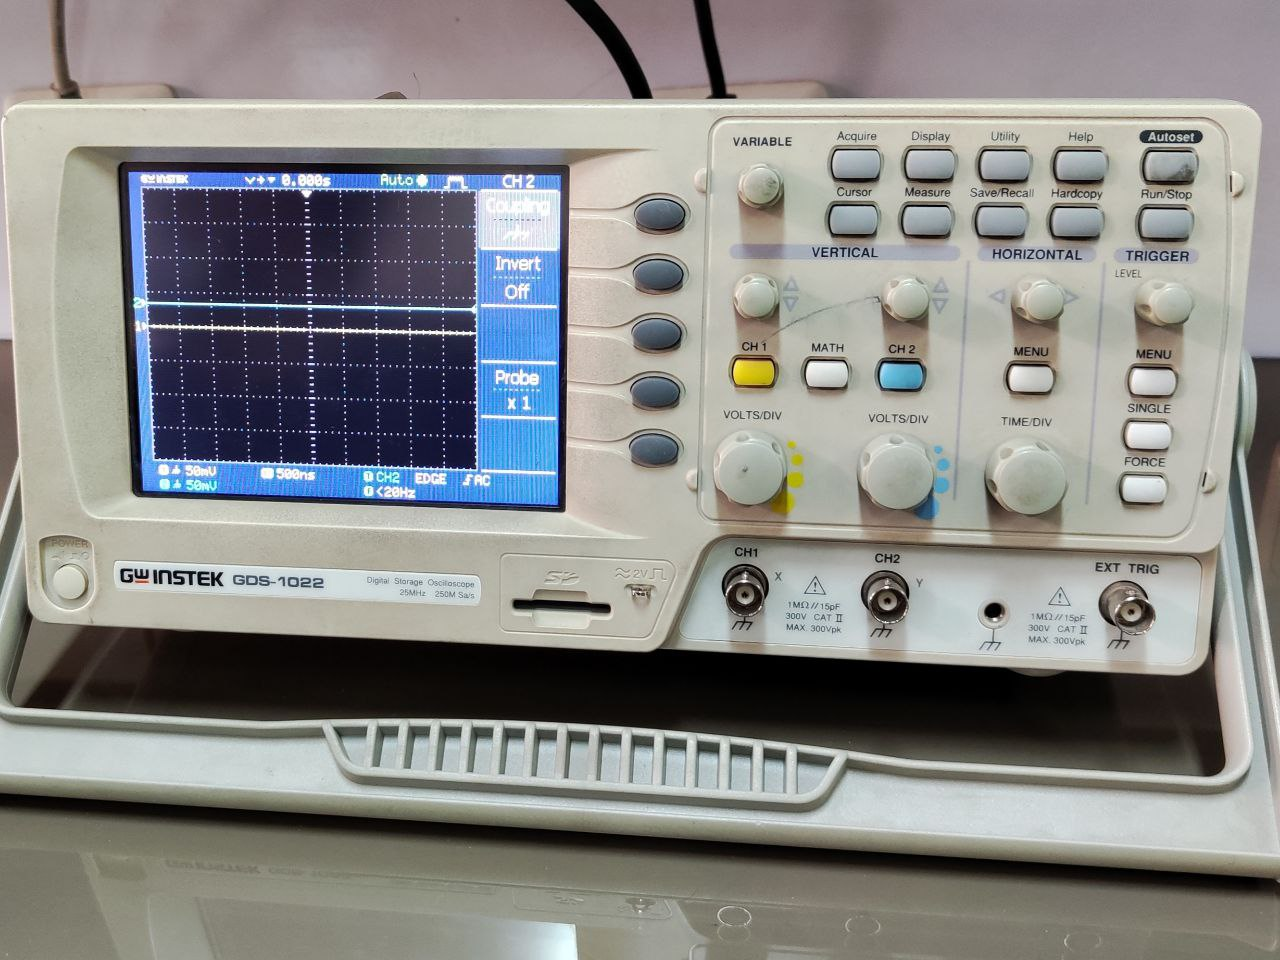
\includegraphics[scale=\PicScale]{Fig/1.jpeg}
                \caption{Oscilloscope's front view.}
            \end{center}
        \end{figure}
        \begin{figure}[H]
            \begin{center}
                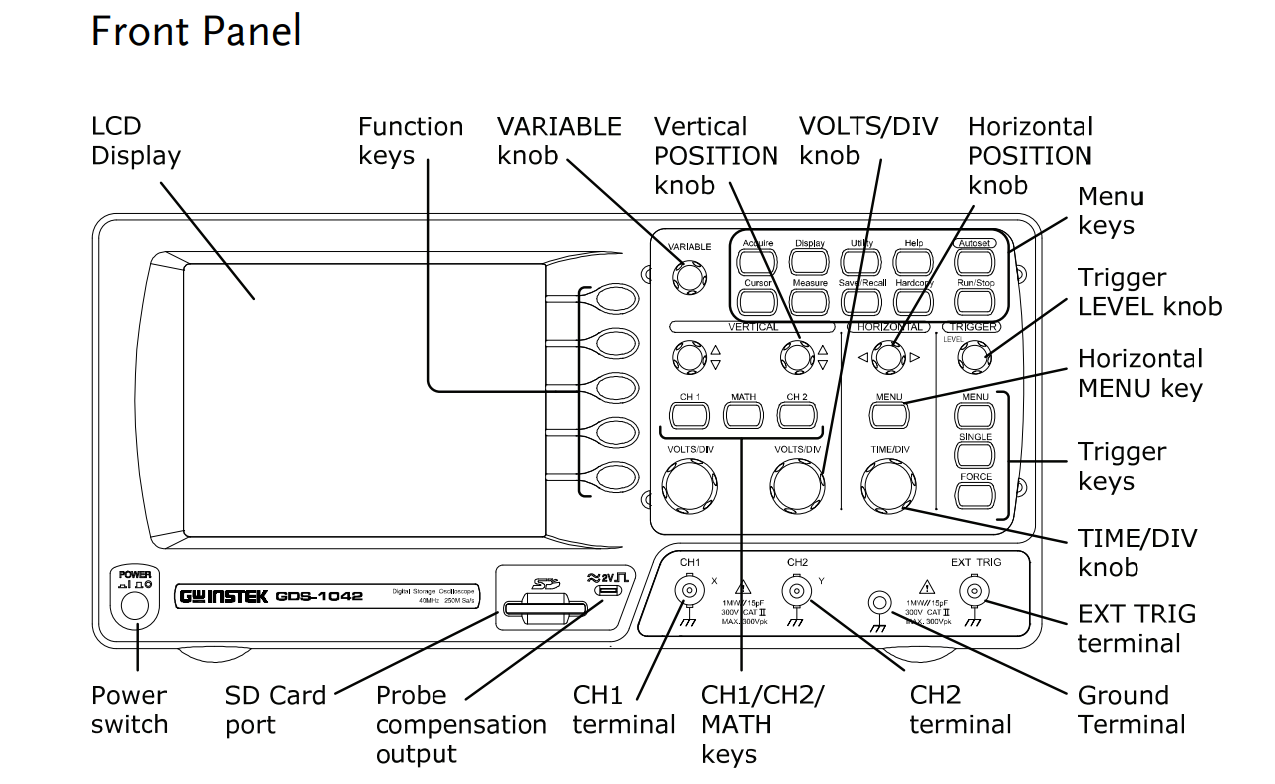
\includegraphics[scale=0.5]{Fig/30.png}
                \caption{Oscilloscope's front panel buttons .}
            \end{center}
        \end{figure}

        \paragraph*{Display group:}
        Display group includes lcd display and function buttons: \\
        $1$- LCD display which is TFT color, 320 x 234 resolution, wide angle view LCD display.   \\
        $2$- Function keys(F1 (top) to F5 (bottom)): Are used to Activate the functions which
        appear in the left side of the LCD display. \\

        \paragraph*{Vertical group:}
        Vertical group Includes following buttons and controllers: \\
        $1$- Vertical position knob: Is used to move the waveform vertically. \\
        $2$- VOLTS/DIV knob: Is used to select the vertical scale for the signal. \\
        $3$- CH1/CH2 key: Are used to configure the vertical scale and coupling mode for each channel. \\
        $4$- MATH key: Is used to perform math operations.

        \paragraph*{Horizontal group:}
        Horizontal group Includes following buttons and controllers: \\
        $1$- Horizontal position knob: Is used to moves the waveform horizontally. \\
        $2$- Horizontal menu key: Is used to configures the horizontal view. \\
        $3$- TIME/DIV knob: Is used to select the horizontal scale. \\

        \paragraph*{Trigger group:}
        Trigger group Includes following buttons and controllers: \\
        $1$- Trigger level knob: Is used to set the trigger level.Using the trigger level knob moves the trigger point up or down.  \\
        $2$- Single trigger key: Is used to select the single trigger mode \\
        $3$- Trigger force key: Is used to acquire the input signal once regardless of the trigger condition at the time. \\
    }

\end{question}

%----------------------------------------------------------------------------------------
%	QUESTION 2
%----------------------------------------------------------------------------------------

\begin{question}

    \questiontext{Turn on the oscilloscope and set its channels to GND input mode. Use vertical position knobs to move and adjust the ground levels. }

    \answer{

        \begin{figure}[H]
            \begin{center}
                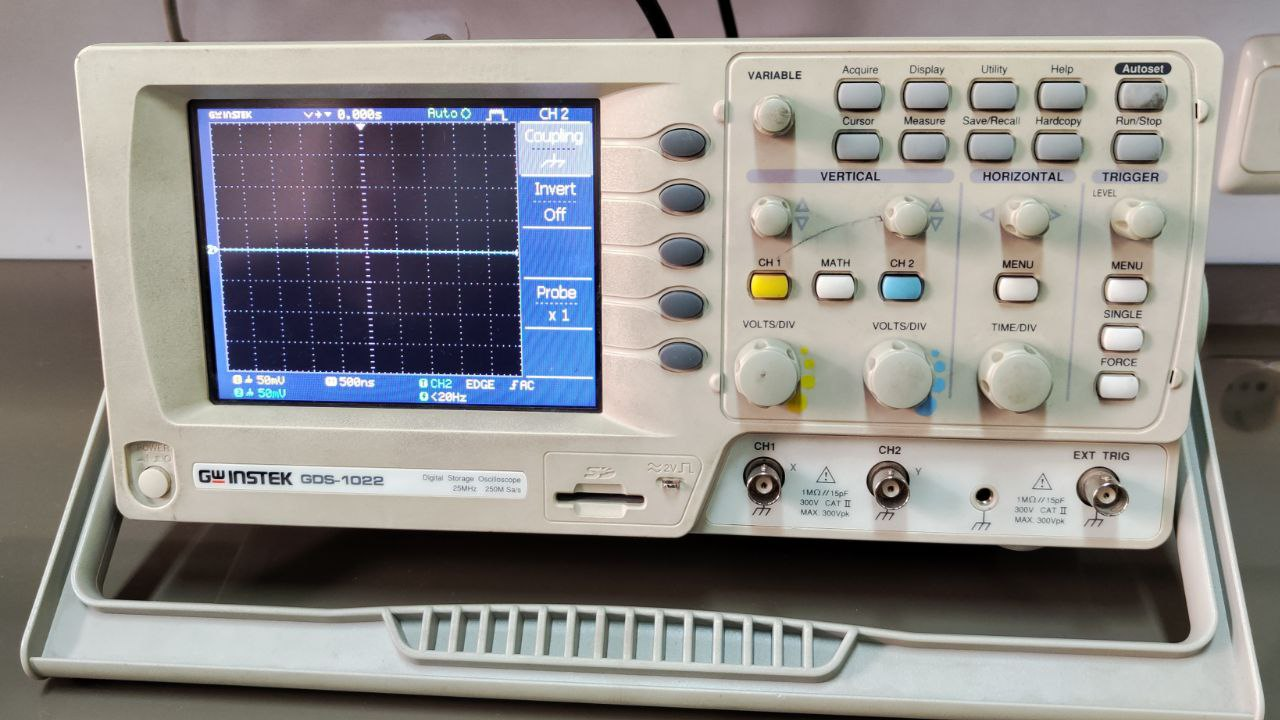
\includegraphics[scale=\PicScale]{Fig/2.jpeg}
                \caption{Channel 2 adjusted.}
            \end{center}
        \end{figure}

        \begin{figure}[H]
            \begin{center}
                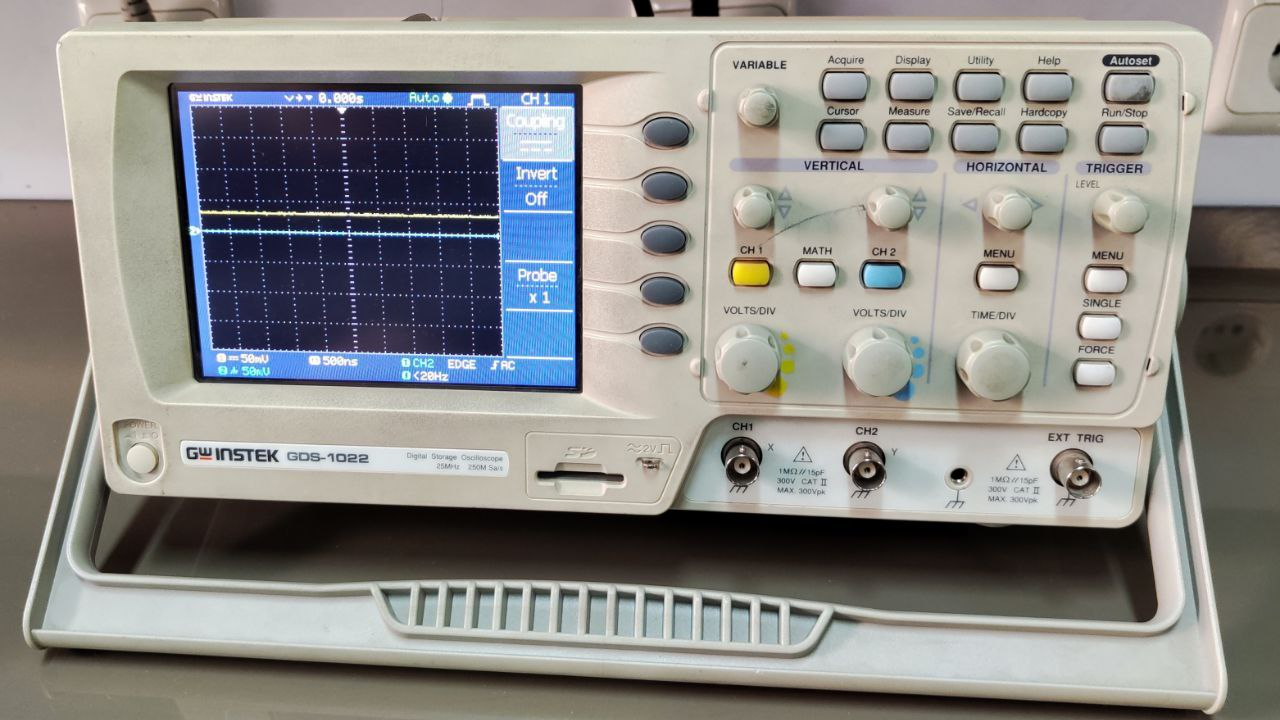
\includegraphics[scale=\PicScale]{Fig/3.jpeg}
                \caption{Both channels adjusted.}
            \end{center}
        \end{figure}

    }

\end{question}


%----------------------------------------------------------------------------------------
%	QUESTION 3
%----------------------------------------------------------------------------------------

\begin{question}

    \questiontext{Set the first channel to DC input mode while no signal is fed to its probe. Watch how the horizontal axis is swept. Change the time/div knob and see its impact on the sweep speed. }

    \answer{

        \begin{figure}[H]
            \begin{center}
                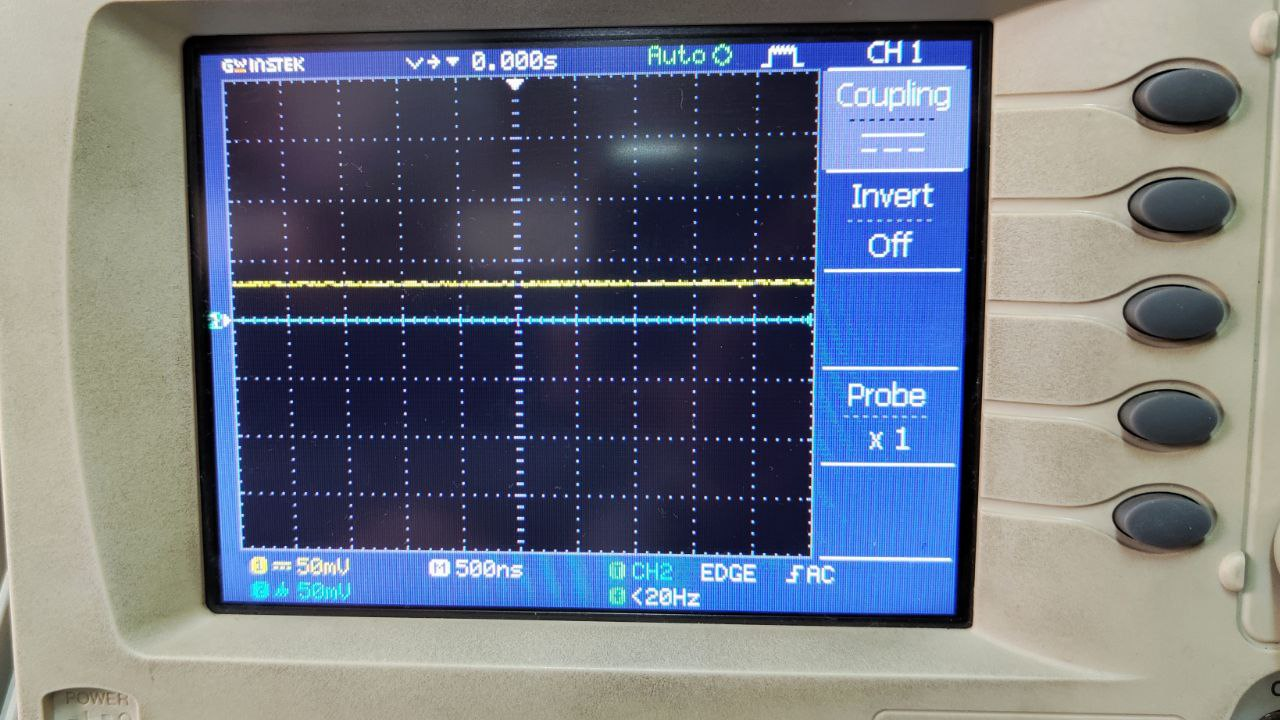
\includegraphics[scale=\PicScale]{Fig/4.jpeg}
                \caption{first channel DC mode.}
            \end{center}
        \end{figure}

        \begin{figure}[H]
            \begin{center}
                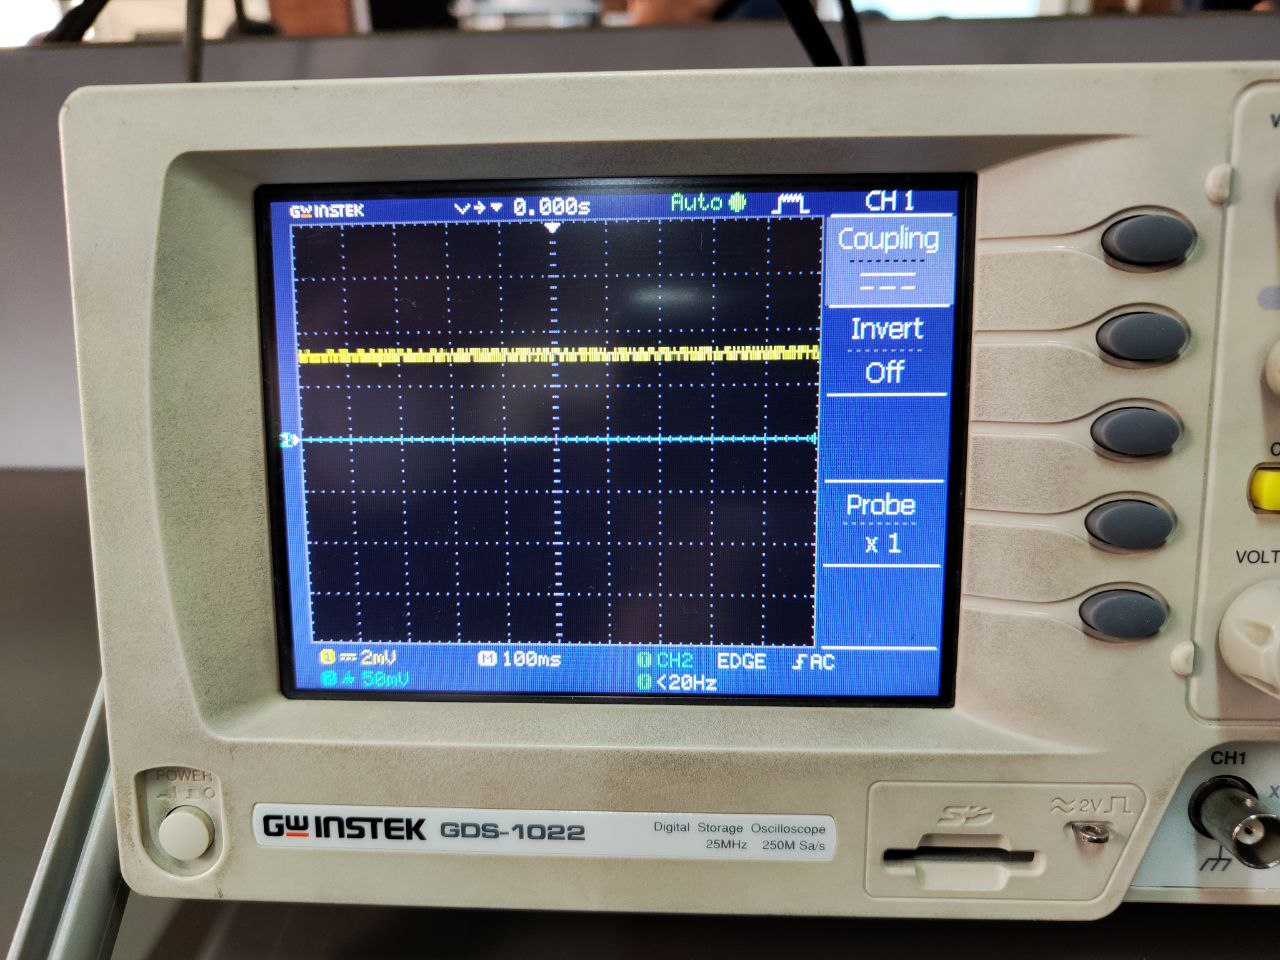
\includegraphics[scale=\PicScale]{Fig/5.jpeg}
                \caption{time/div set to 100ms.}
            \end{center}
        \end{figure}

        \begin{figure}[H]
            \begin{center}
                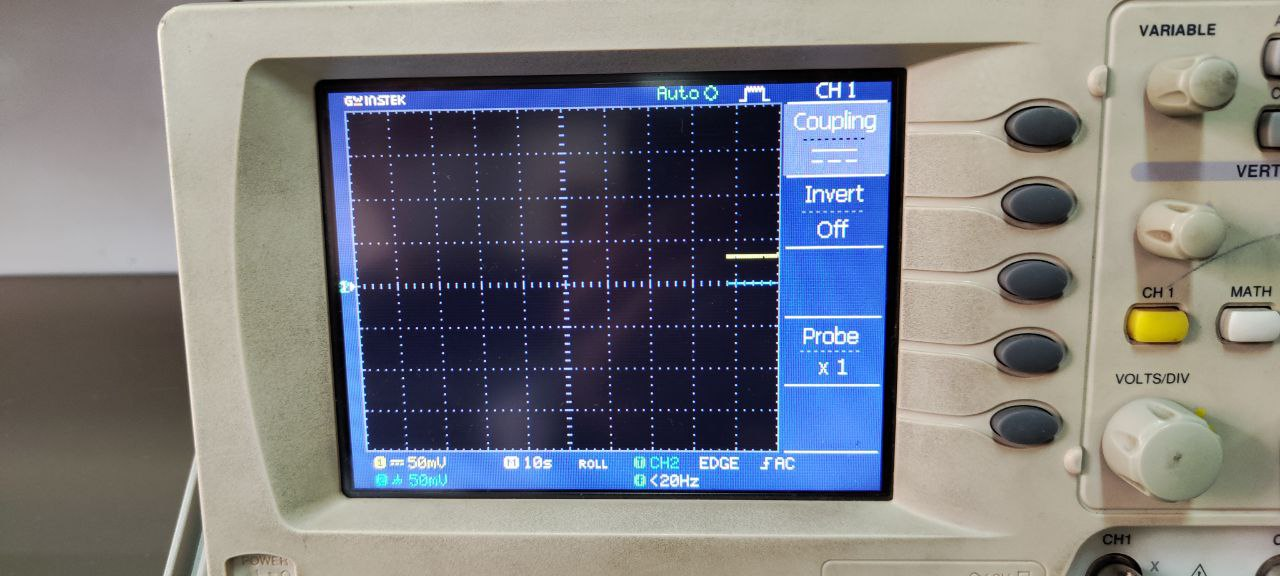
\includegraphics[scale=\PicScale]{Fig/6.jpeg}
                \caption{time/div set to 10s.}
            \end{center}
        \end{figure}

    }

\end{question}

%----------------------------------------------------------------------------------------
%	QUESTION 4
%----------------------------------------------------------------------------------------

\begin{question}

    \questiontext{Connect a probe to the oscilloscope and set the volt/div knob to its minimum. Touch the probe tip by your finger. What do see on the oscilloscope screen? Change in input mode to AC, DC, and GND and check the results.}

    \answer{

        \begin{figure}[H]
            \begin{center}
                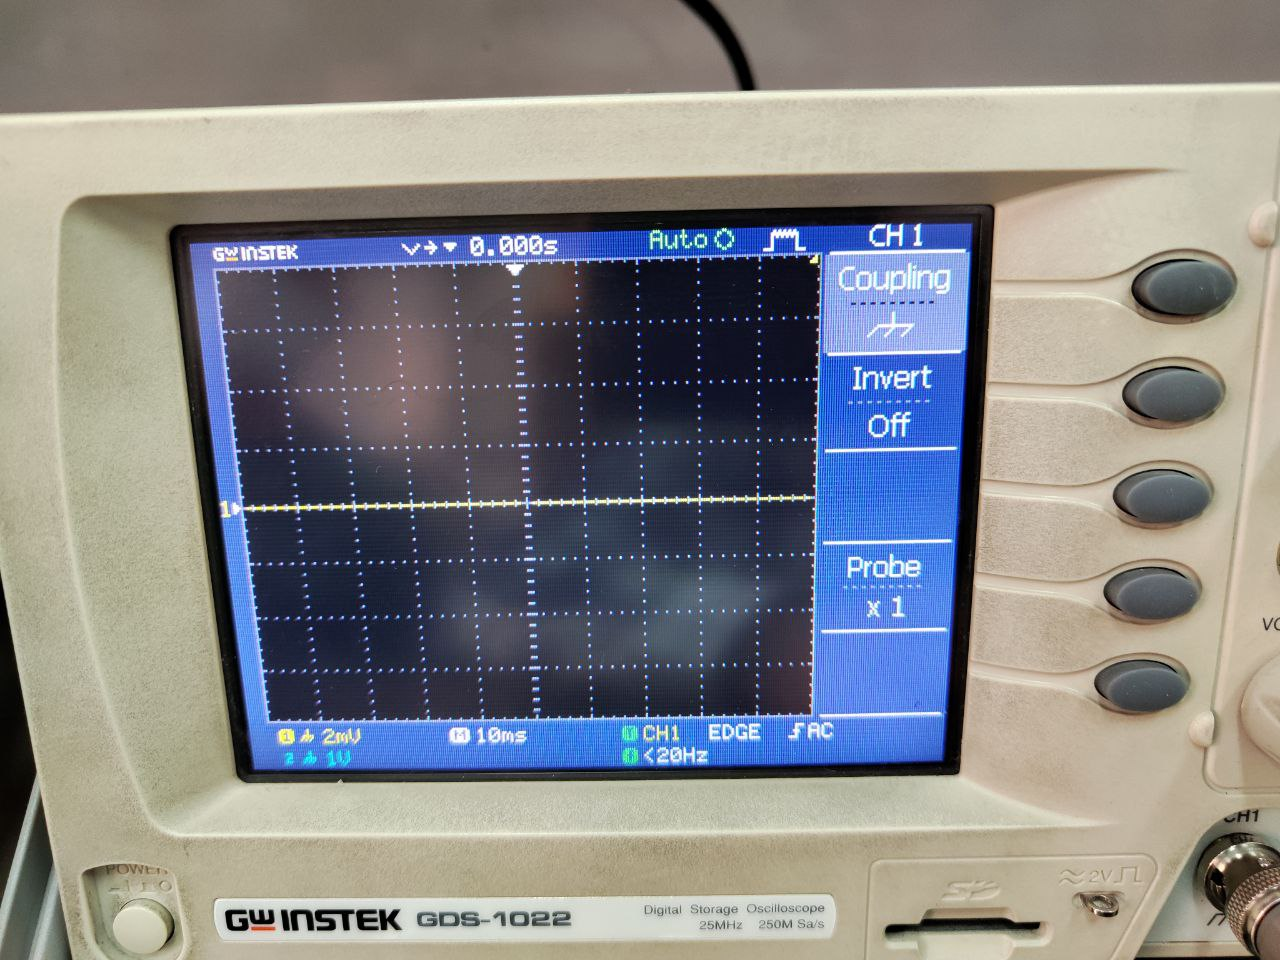
\includegraphics[scale=\PicScale]{Fig/7.jpeg}
                \caption{input mode set to GND.}
            \end{center}
        \end{figure}

        \begin{figure}[H]
            \begin{center}
                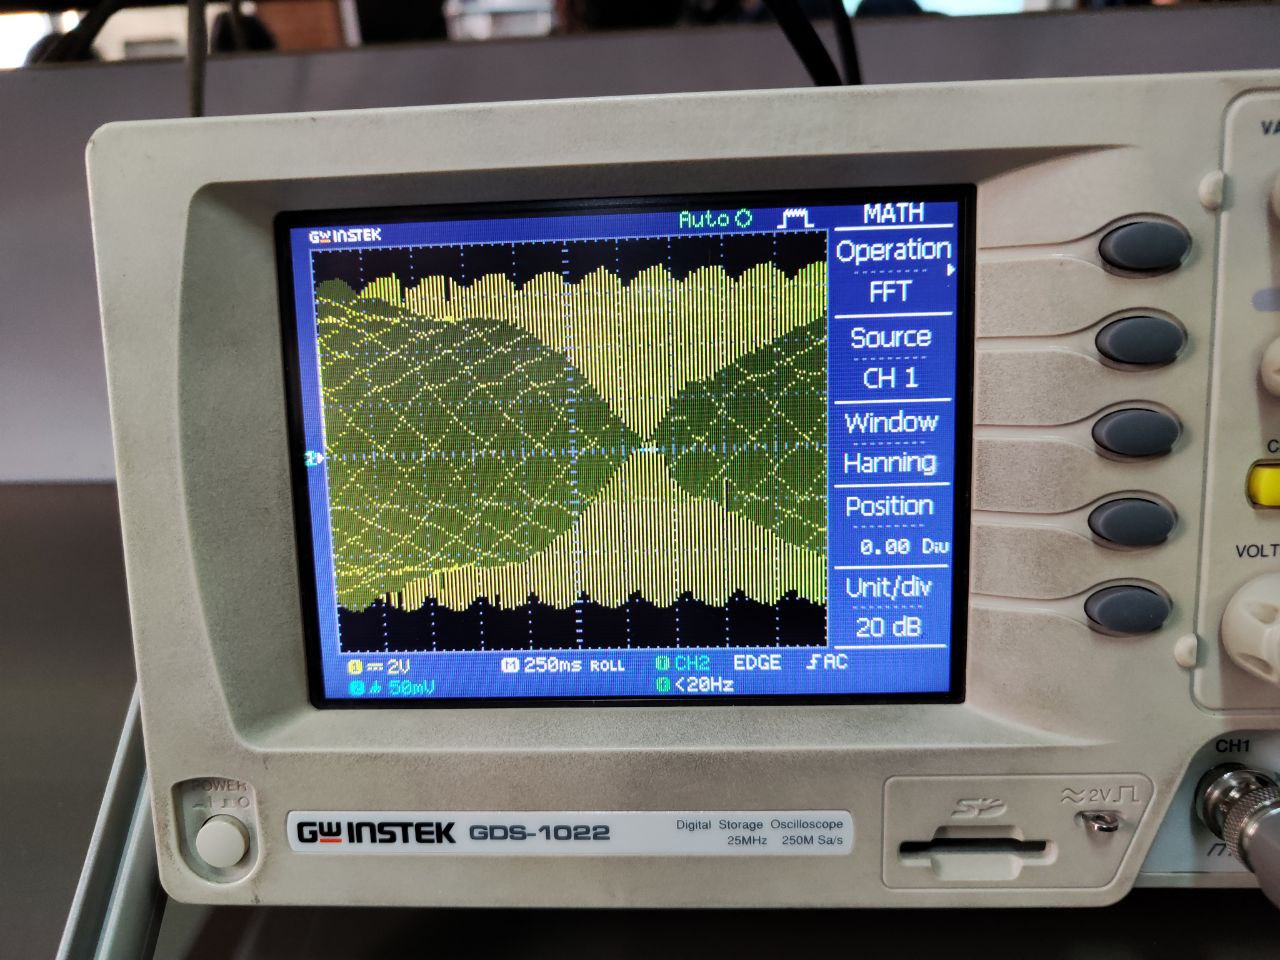
\includegraphics[scale=\PicScale]{Fig/8.jpeg}
                \caption{input mode set to AC.}
            \end{center}
        \end{figure}

        \begin{figure}[H]
            \begin{center}
                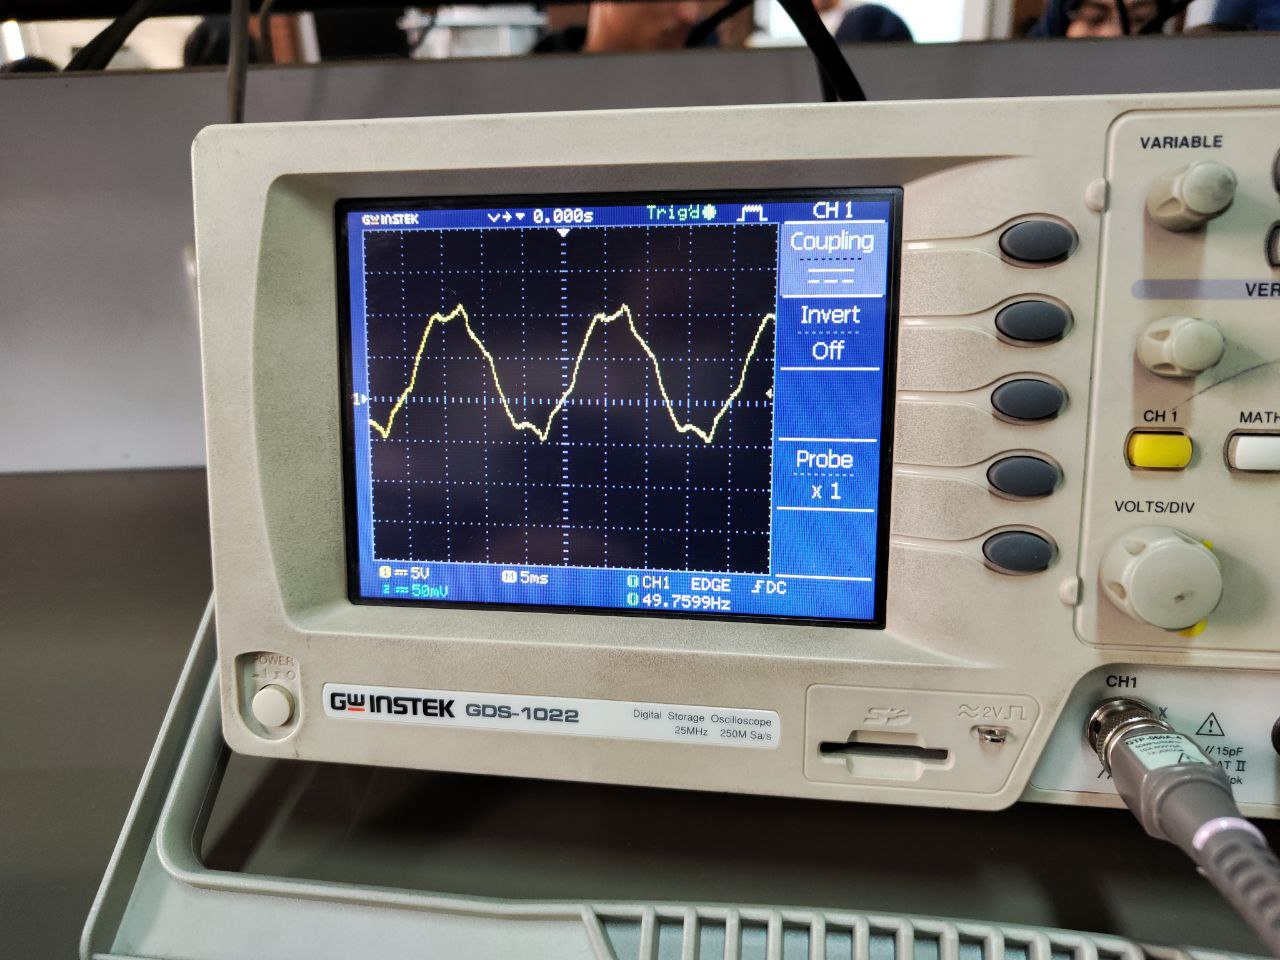
\includegraphics[scale=\PicScale]{Fig/9.jpeg}
                \caption{input mode set to DC.}
            \end{center}
        \end{figure}

    }

\end{question}

%----------------------------------------------------------------------------------------
%	QUESTION 5
%----------------------------------------------------------------------------------------

\begin{question}

    \questiontext{Connect a proper probe to the first channel of the oscilloscope and watch the calibrated signal of the built-in frequency generator. Read the frequency and amplitude of the calibrated signal. How can this signal be used for calibration check? What happens when the probe is set to 10X?}

    \answer{

        \begin{figure}[H]
            \begin{center}
                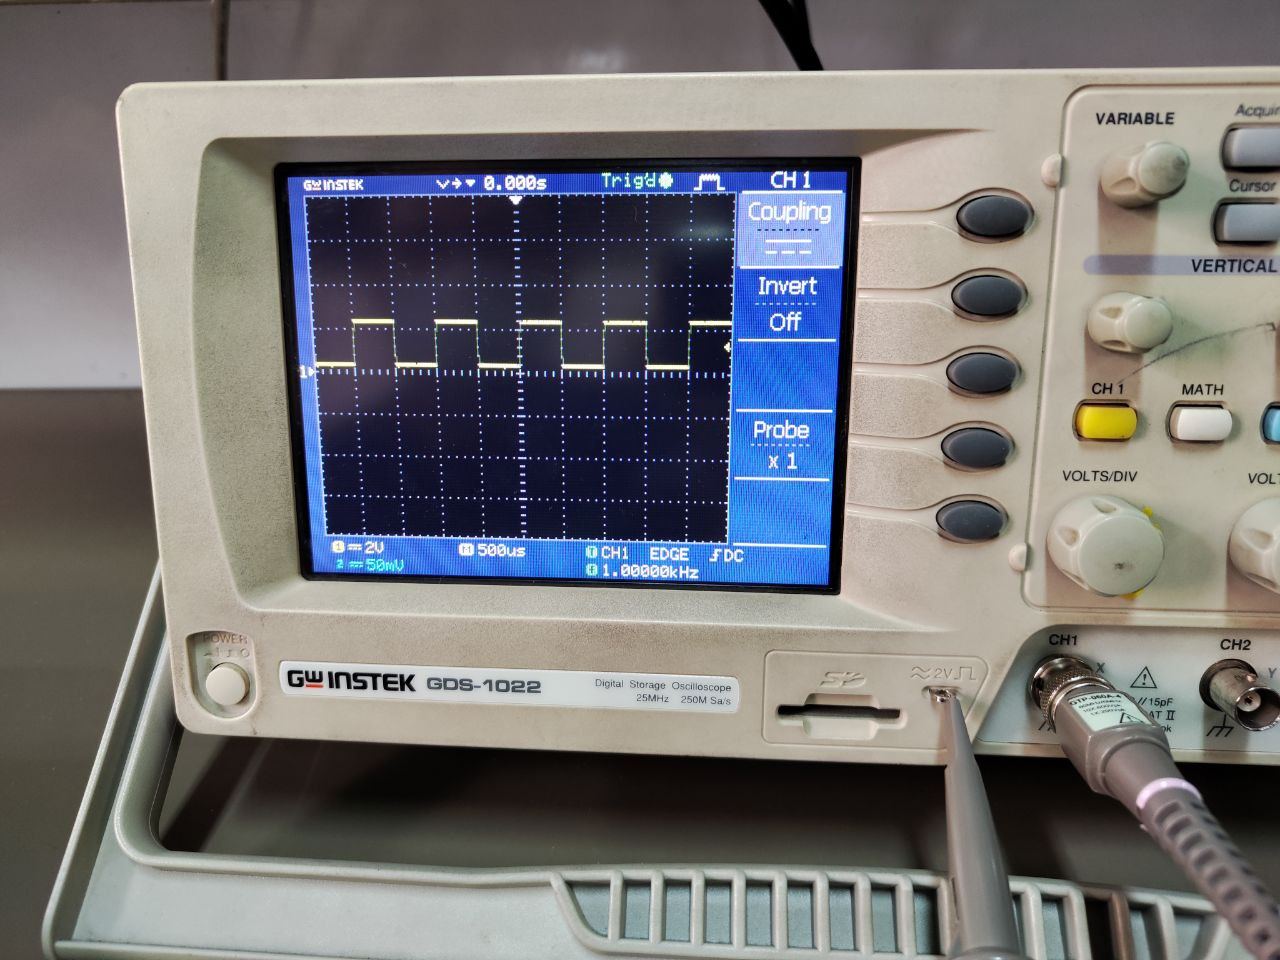
\includegraphics[scale=\PicScale]{Fig/10.jpeg}
                \caption{first channel connected to the oscilloscope calibrated signal
                    generator.Pay attention to the channel error.}
            \end{center}
        \end{figure}

        \begin{figure}[H]
            \begin{center}
                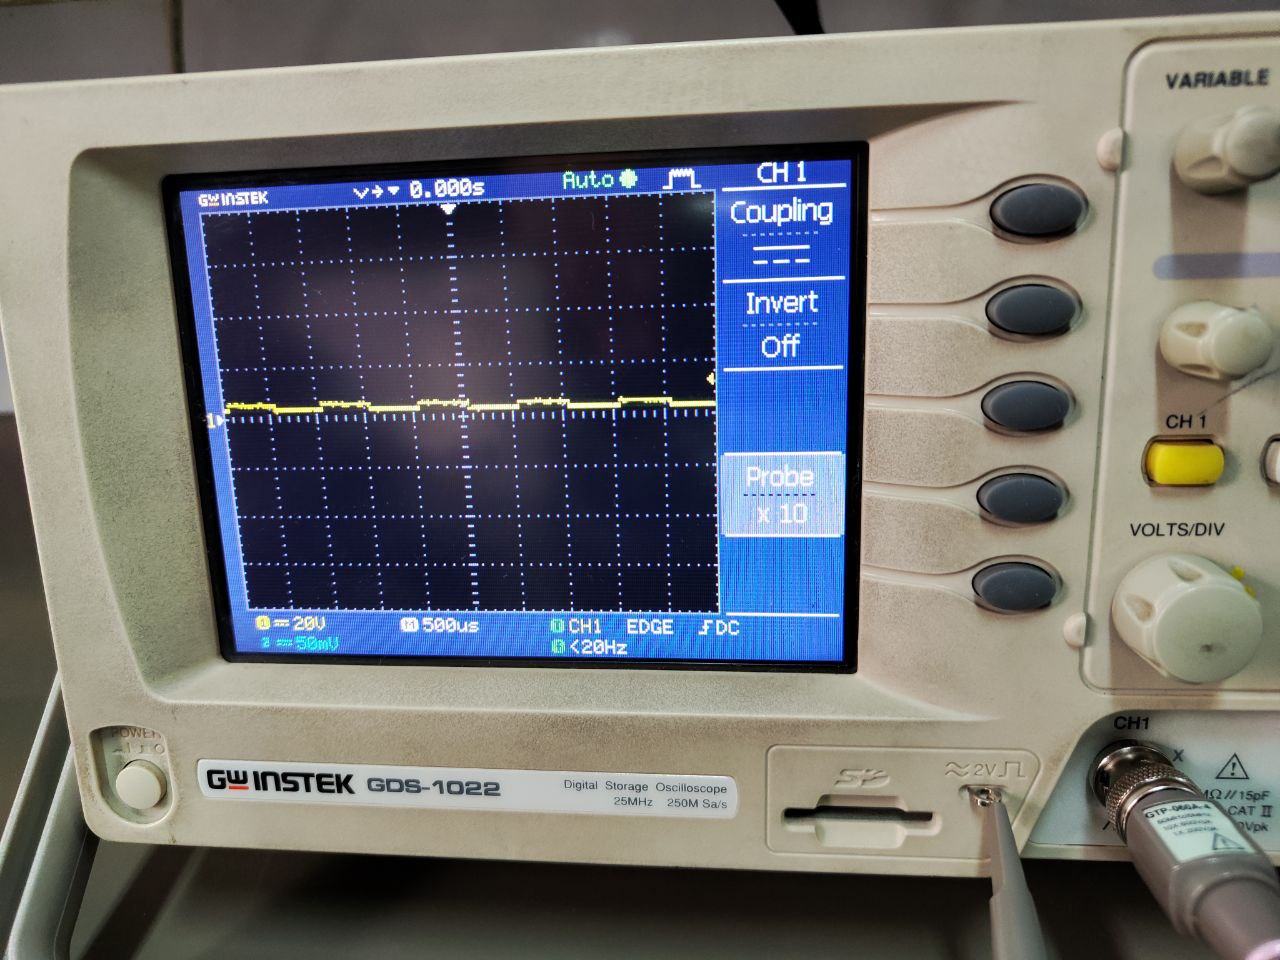
\includegraphics[scale=\PicScale]{Fig/11.jpeg}
                \caption{Probe set to 10X.}
            \end{center}
        \end{figure}

        \paragraph*{}
        The frequency and amplitude of the calibrated signal are $1$ KHz and $1$ V respectively. This signal can be used for calibration check by comparing the signal with the calibrated signal.
        When the probe is set to 10X, the amplitude of the signal is reduced by a factor of 10.

    }

\end{question}

%----------------------------------------------------------------------------------------
%	QUESTION 6
%----------------------------------------------------------------------------------------

\begin{question}

    \questiontext{Set the controls of the function generator to produce a sine wave of $1$ kHz frequency and $2$ V amplitude. Use the oscilloscope to see the signal. Read the frequency and amplitude of the sine wave. Is there any difference between the read and set frequencies? Why?}

    \answer{

        \begin{figure}[H]
            \begin{center}
                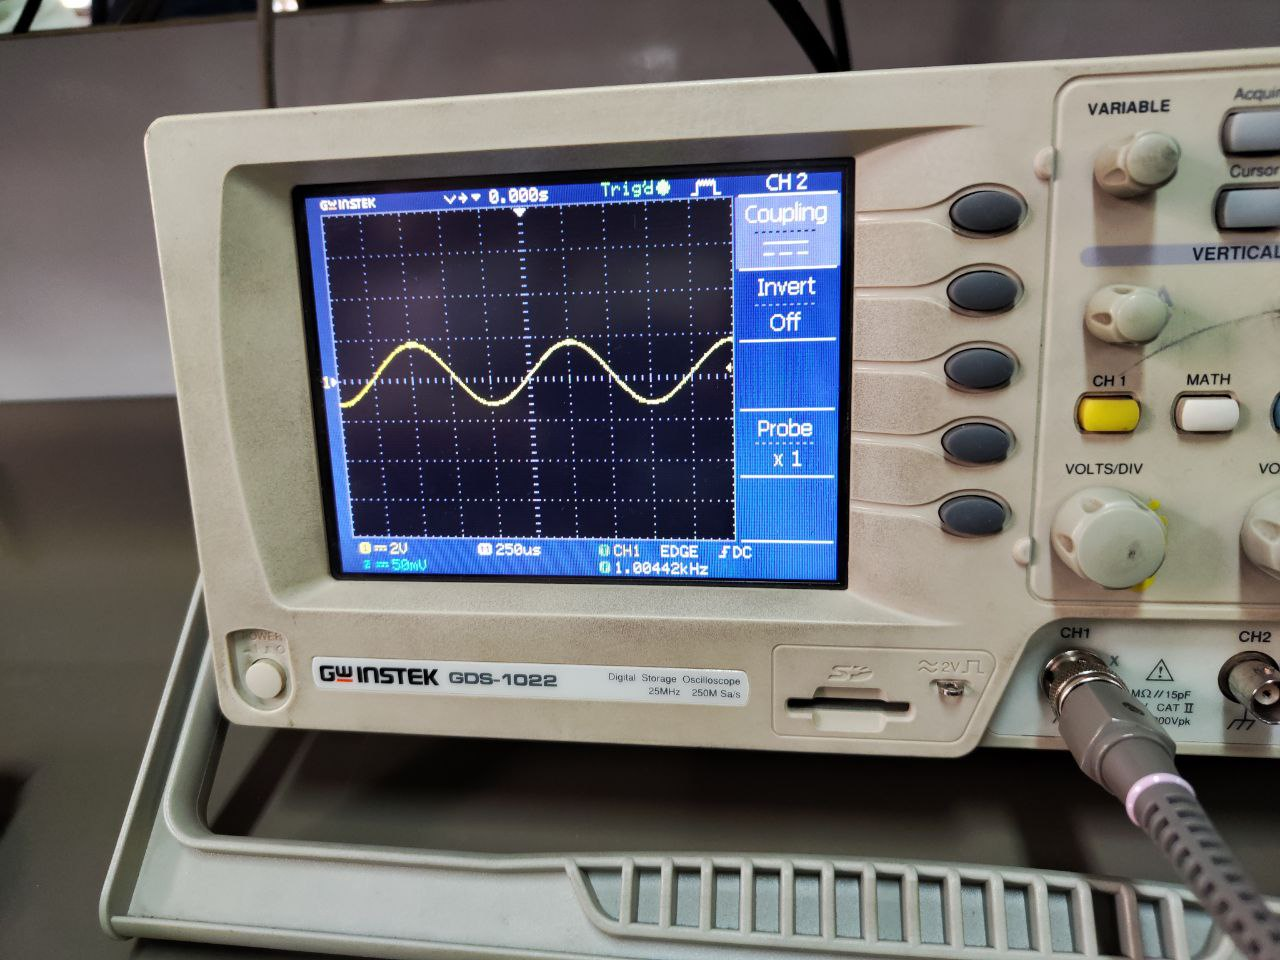
\includegraphics[scale=\PicScale]{Fig/12.jpeg}
                \caption{a sine wave of $1$ kHz frequency and $2$ V amplitude.}
            \end{center}
        \end{figure}

        \begin{figure}[H]
            \begin{center}
                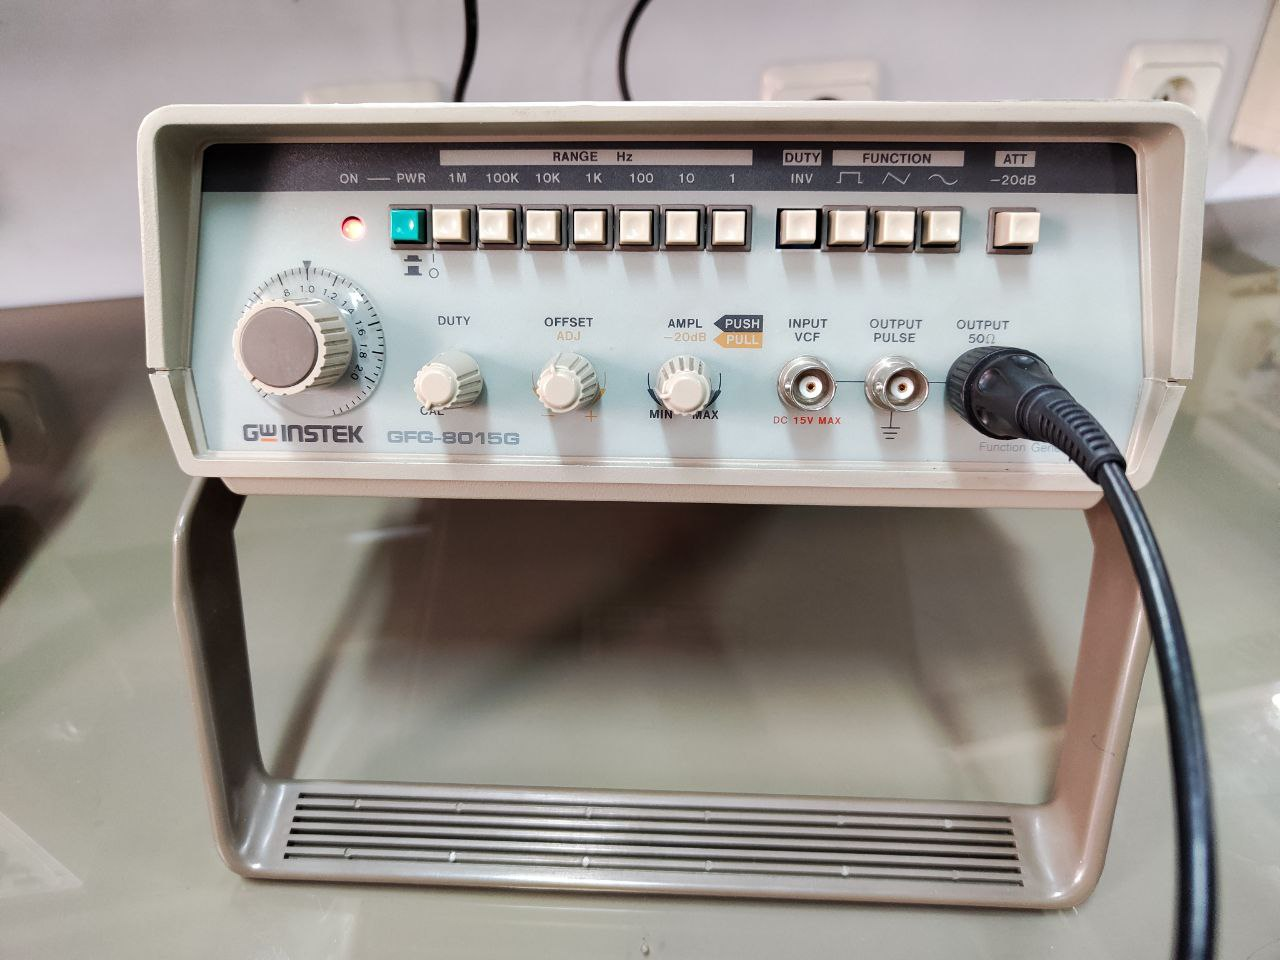
\includegraphics[scale=\PicScale]{Fig/13.jpeg}
                \caption{A picture of the function generator.}
            \end{center}
        \end{figure}

        \paragraph*{}
        The read frequency is $1.004$ KHz and the read amplitude is $2$ V. The difference between the read and set frequencies is due to the errors that might occur in the function generator, during the signal transmission or in the oscilloscope.
         So it's hard to set the frequency and amplitude of the signal exactly the same as wanted.}

\end{question}

%----------------------------------------------------------------------------------------
%	QUESTION 7
%----------------------------------------------------------------------------------------

\begin{question}

    \questiontext{Add a DC offset to the sine wave in the previous part and check the corresponding signal on the oscilloscope screen in different input modes of DC, AC, and GND.}

    \answer{

        \begin{figure}[H]
            \begin{center}
                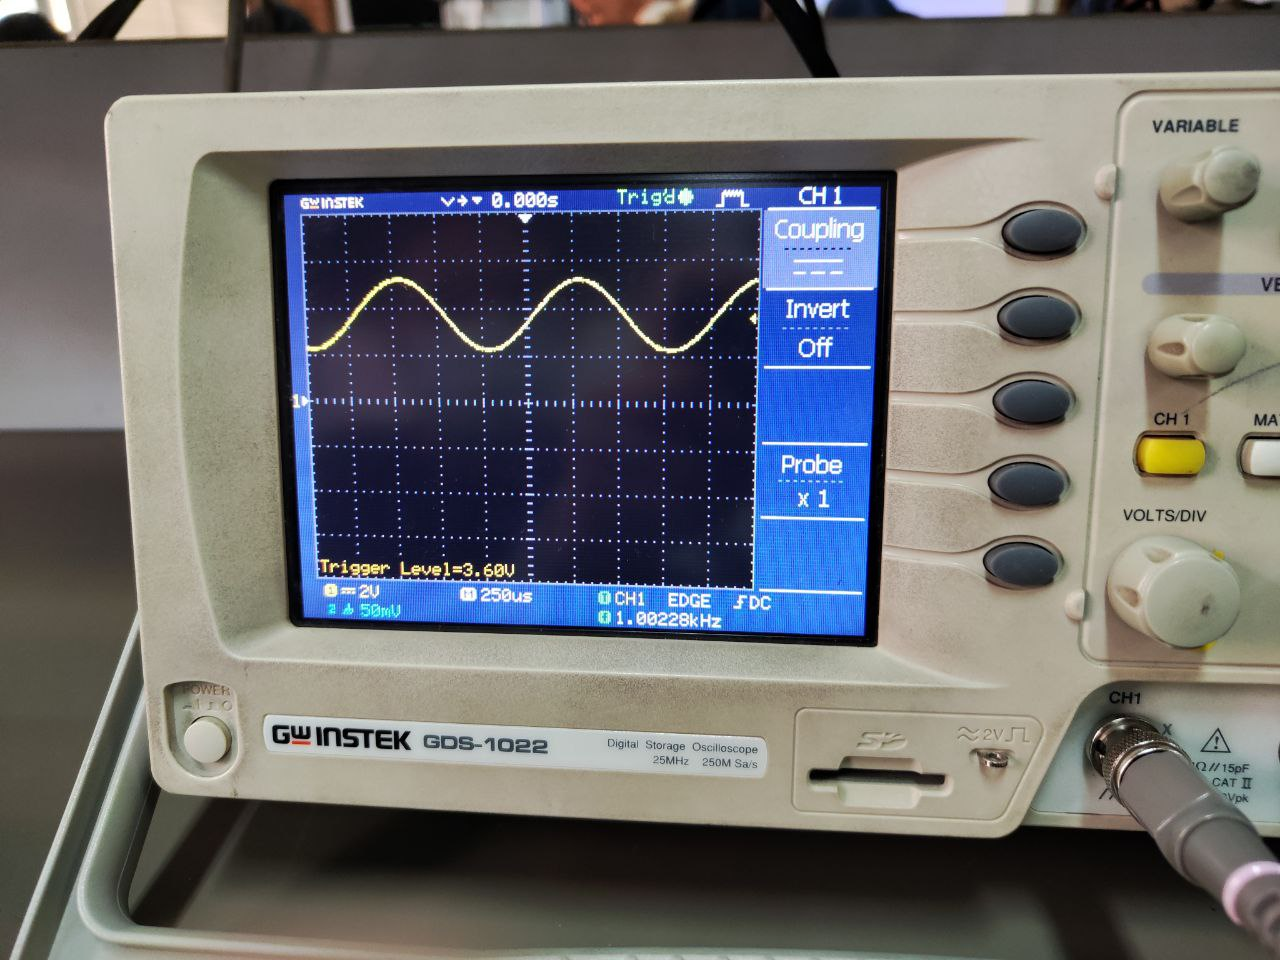
\includegraphics[scale=\PicScale]{Fig/14.jpeg}
                \caption{input mode set to DC.}
            \end{center}
        \end{figure}

        \begin{figure}[H]
            \begin{center}
                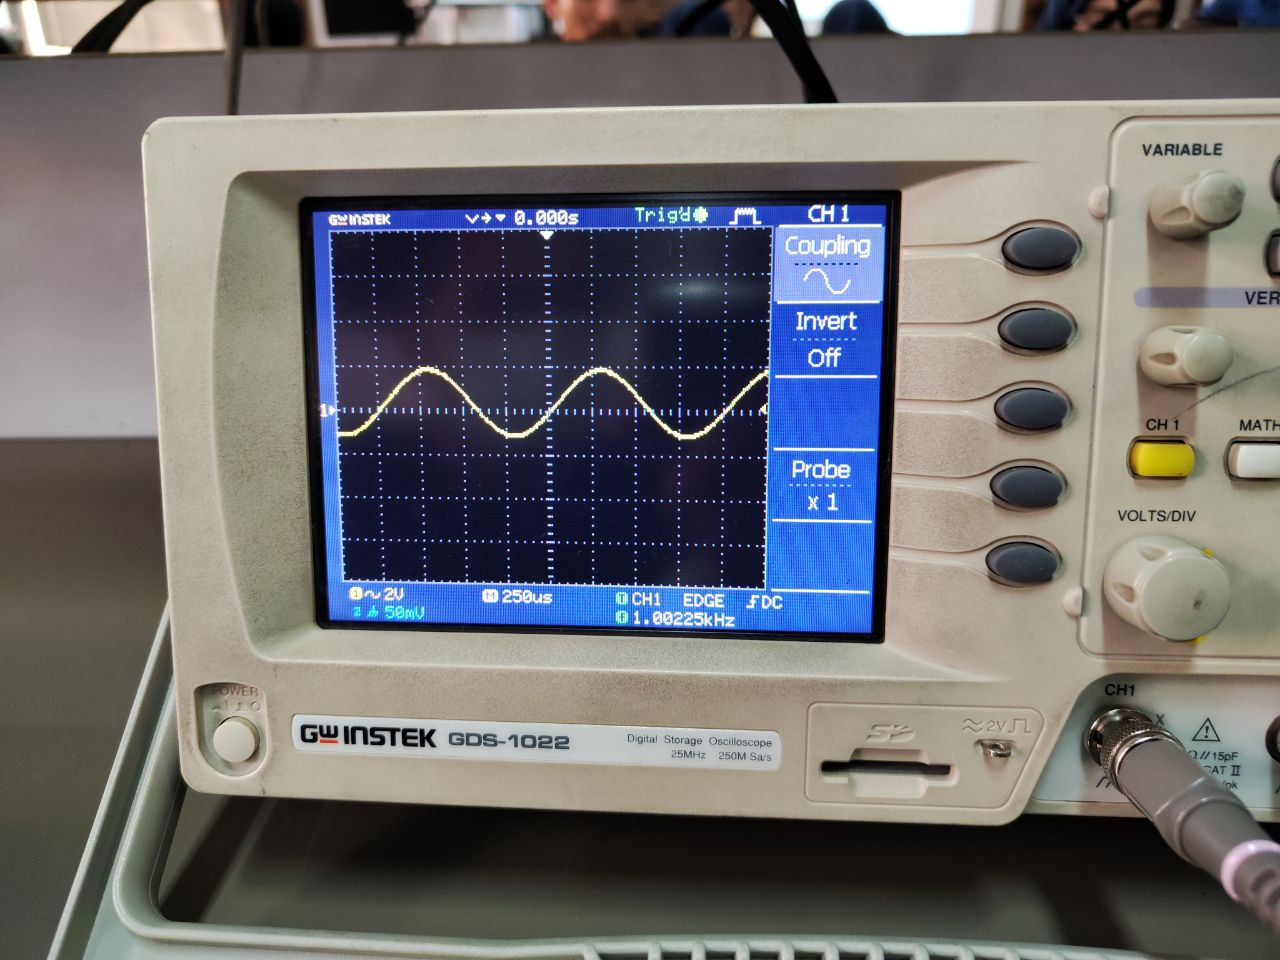
\includegraphics[scale=\PicScale]{Fig/15.jpeg}
                \caption{input mode set to AC.}
            \end{center}
        \end{figure}

        \begin{figure}[H]
            \begin{center}
                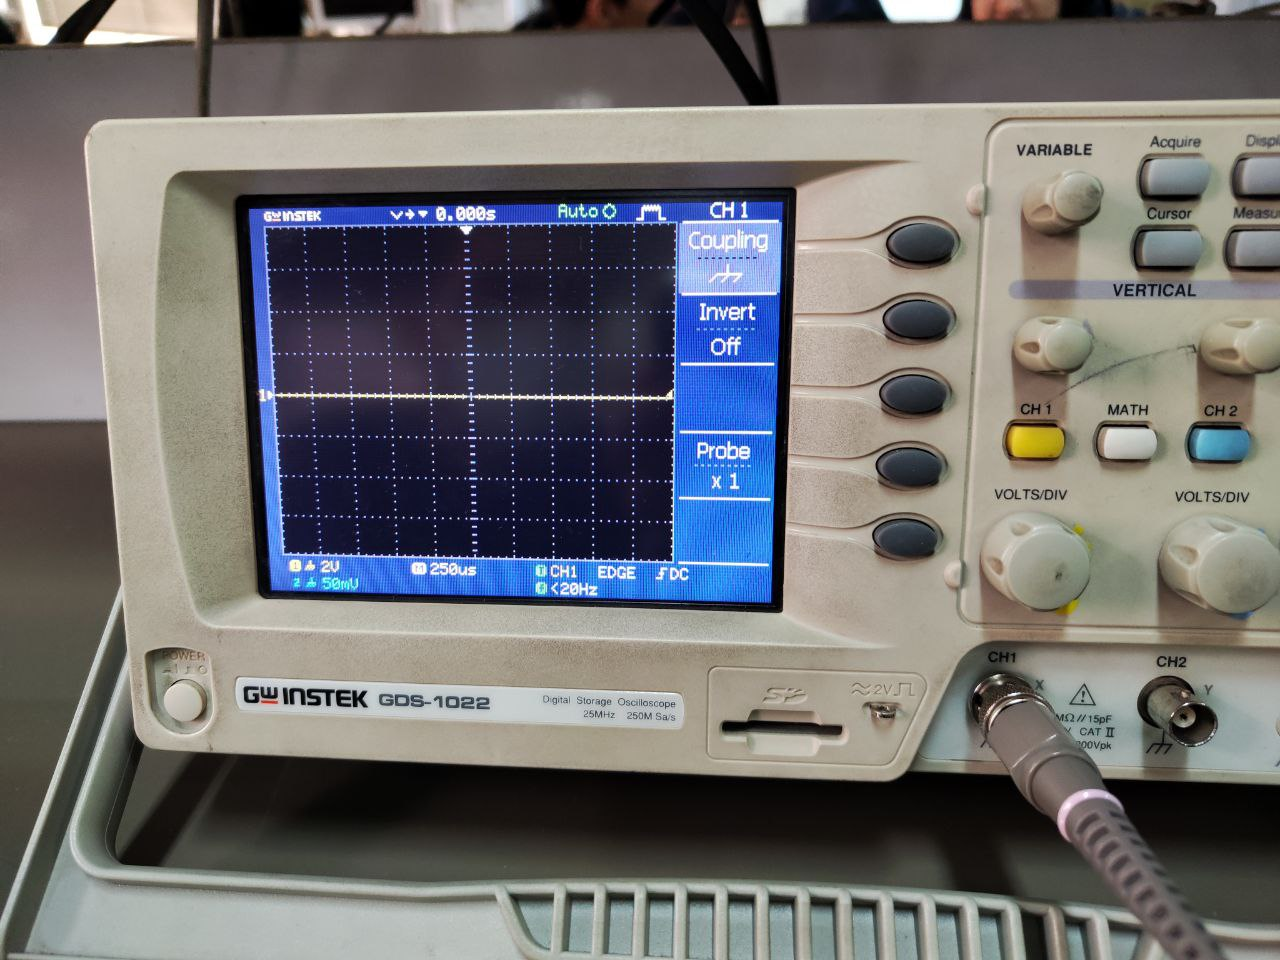
\includegraphics[scale=\PicScale]{Fig/16.jpeg}
                \caption{input mode set to GND.}
            \end{center}
        \end{figure}

        \begin{figure}[H]
            \begin{center}
                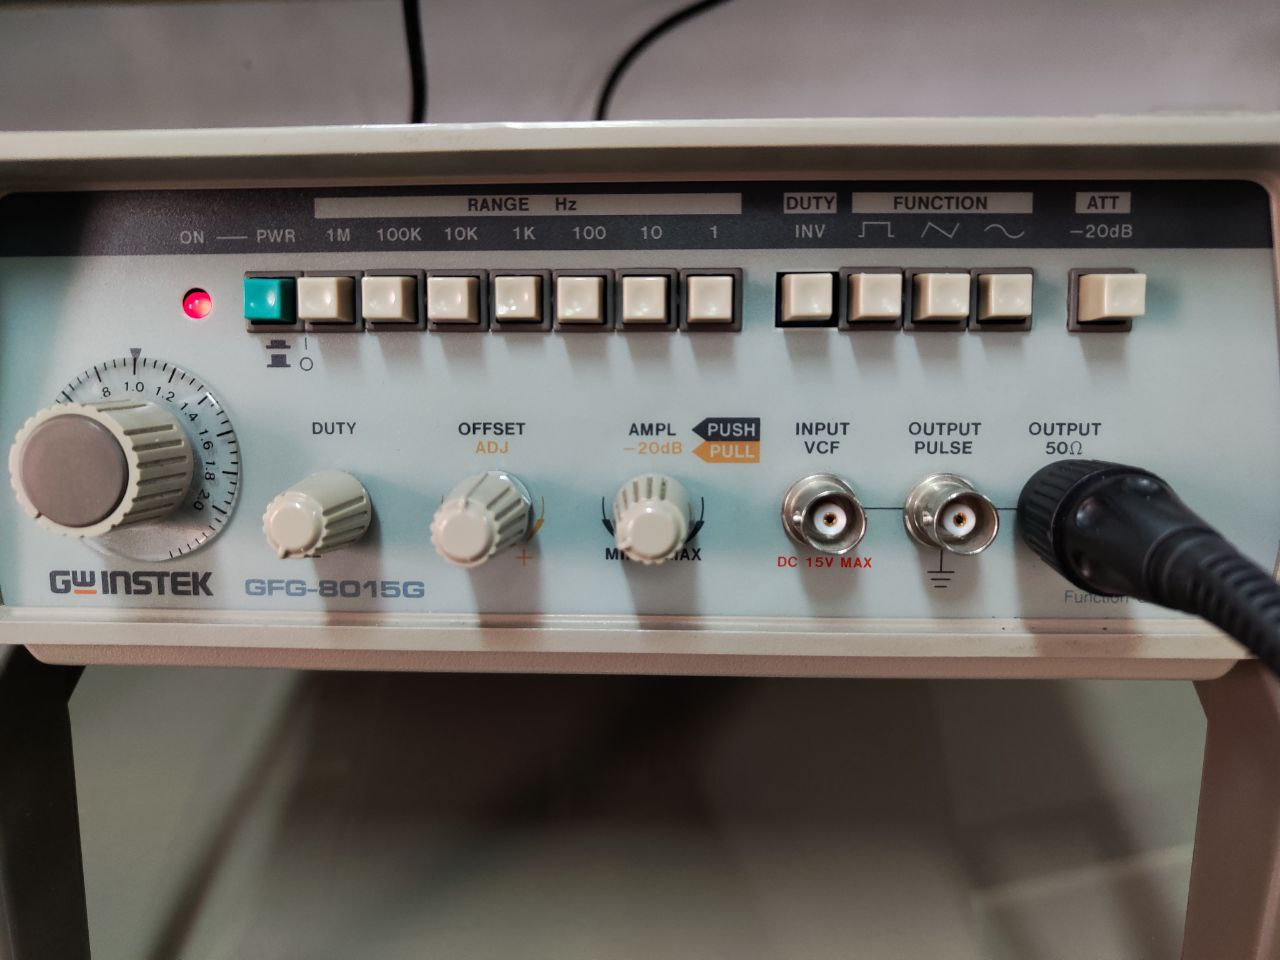
\includegraphics[scale=\PicScale]{Fig/17.jpeg}
                \caption{Function generator offset changed.}
            \end{center}
        \end{figure}

    }

\end{question}

%----------------------------------------------------------------------------------------
%	QUESTION 8
%----------------------------------------------------------------------------------------

\begin{question}

    \questiontext{Feed the two channels of the oscilloscope by a same $1$ KHz sine wave and investigate the functionality of the math operations such as Add and Inv.}

    \answer{

        \begin{figure}[H]
            \begin{center}
                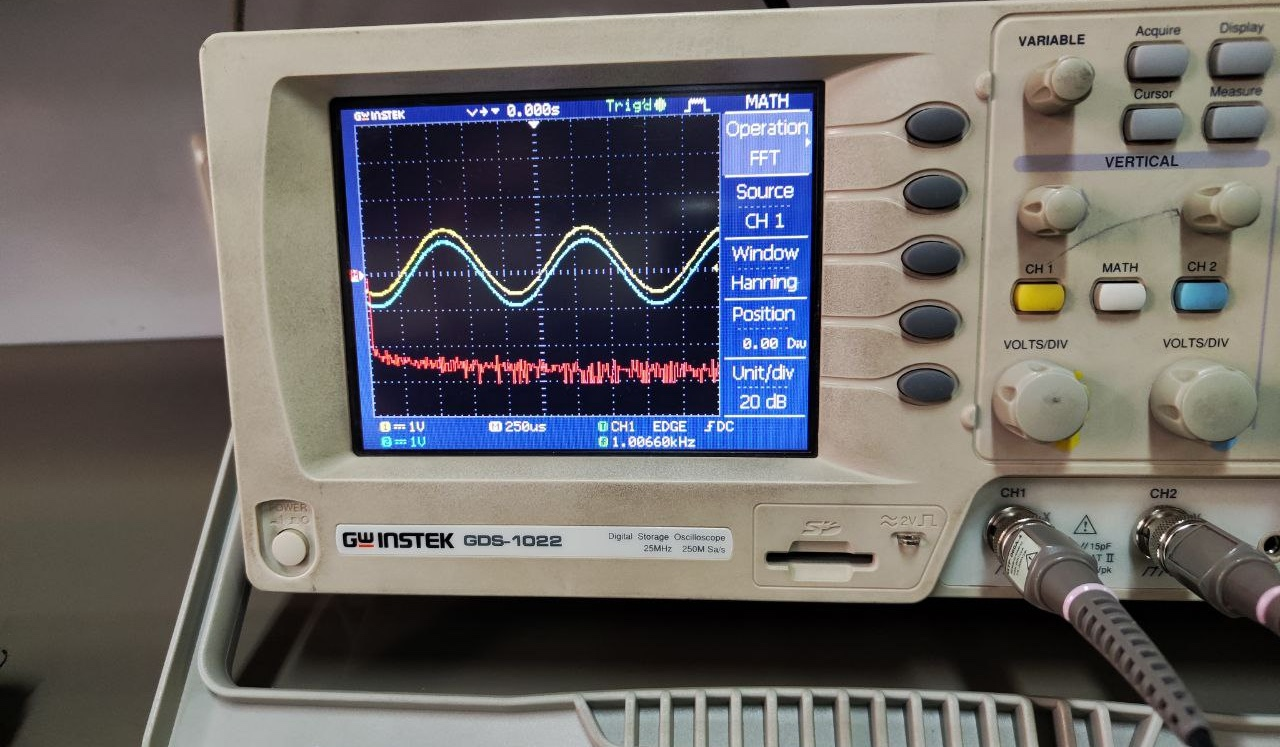
\includegraphics[scale=\PicScale]{Fig/18.jpeg}
                \caption{Both channels are fed with a single function generator. Pay attention to the first channel zero error.}
            \end{center}
        \end{figure}

        \begin{figure}[H]
            \begin{center}
                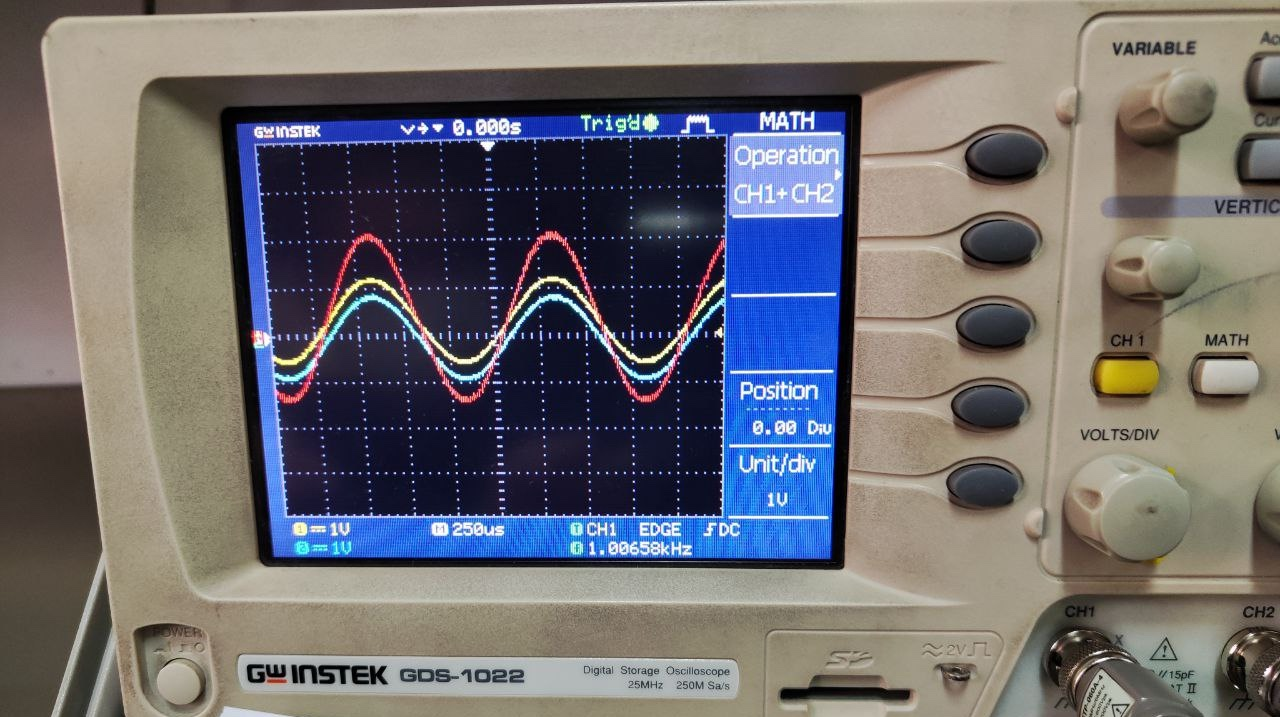
\includegraphics[scale=\PicScale]{Fig/19.jpeg}
                \caption{Add math function.}
            \end{center}
        \end{figure}

        \begin{figure}[H]
            \begin{center}
                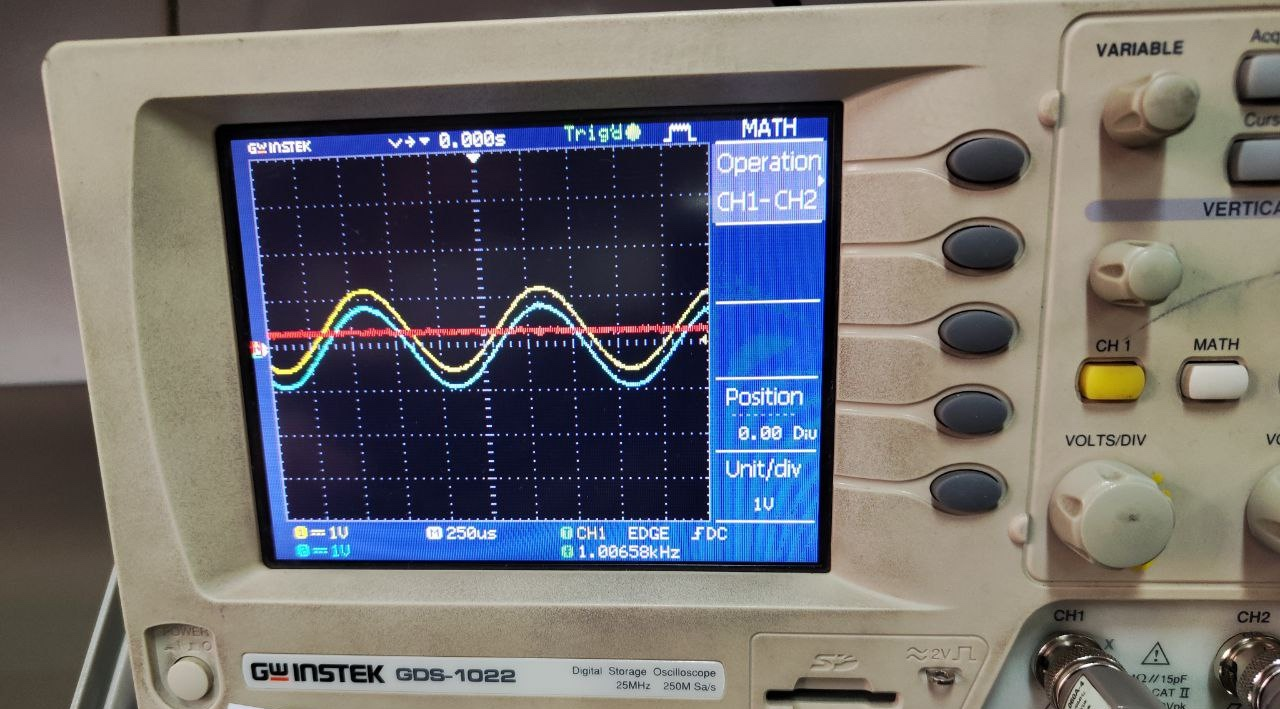
\includegraphics[scale=\PicScale]{Fig/20.jpeg}
                \caption{Inv math function.}
            \end{center}
        \end{figure}

    }

\end{question}

%----------------------------------------------------------------------------------------
%	QUESTION 9
%----------------------------------------------------------------------------------------

\begin{question}

    \questiontext{Repeat the previous part with two $1$ KHz sine waves produced from two different function generators. Explain your observations.}

    \answer{

        \begin{figure}[H]
            \begin{center}
                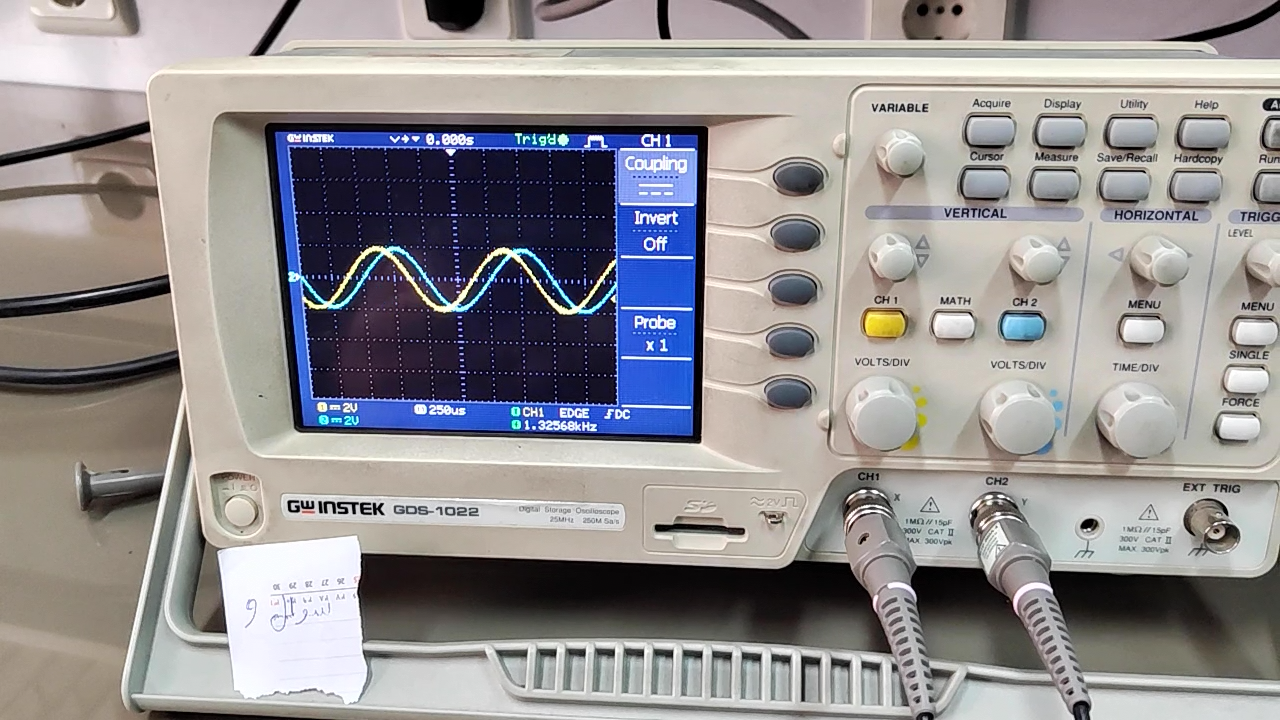
\includegraphics[scale=\PicScale]{Fig/21.png}
                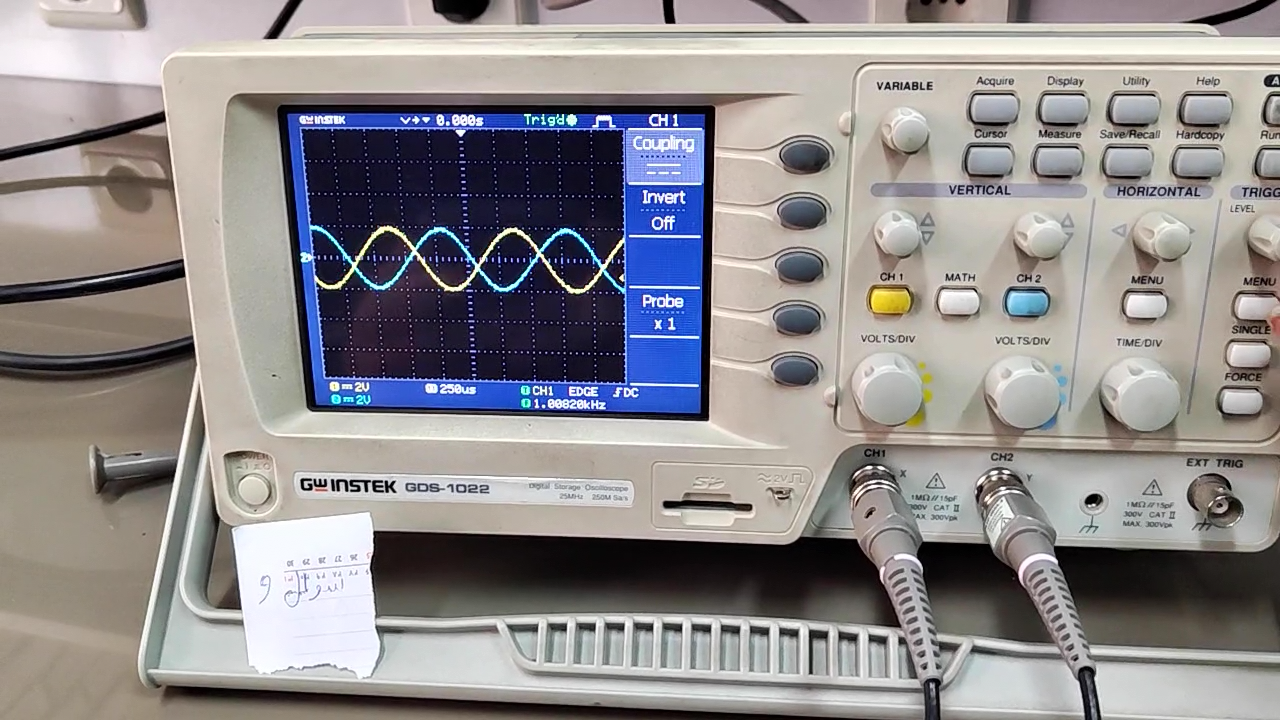
\includegraphics[scale=\PicScale]{Fig/22.png}
                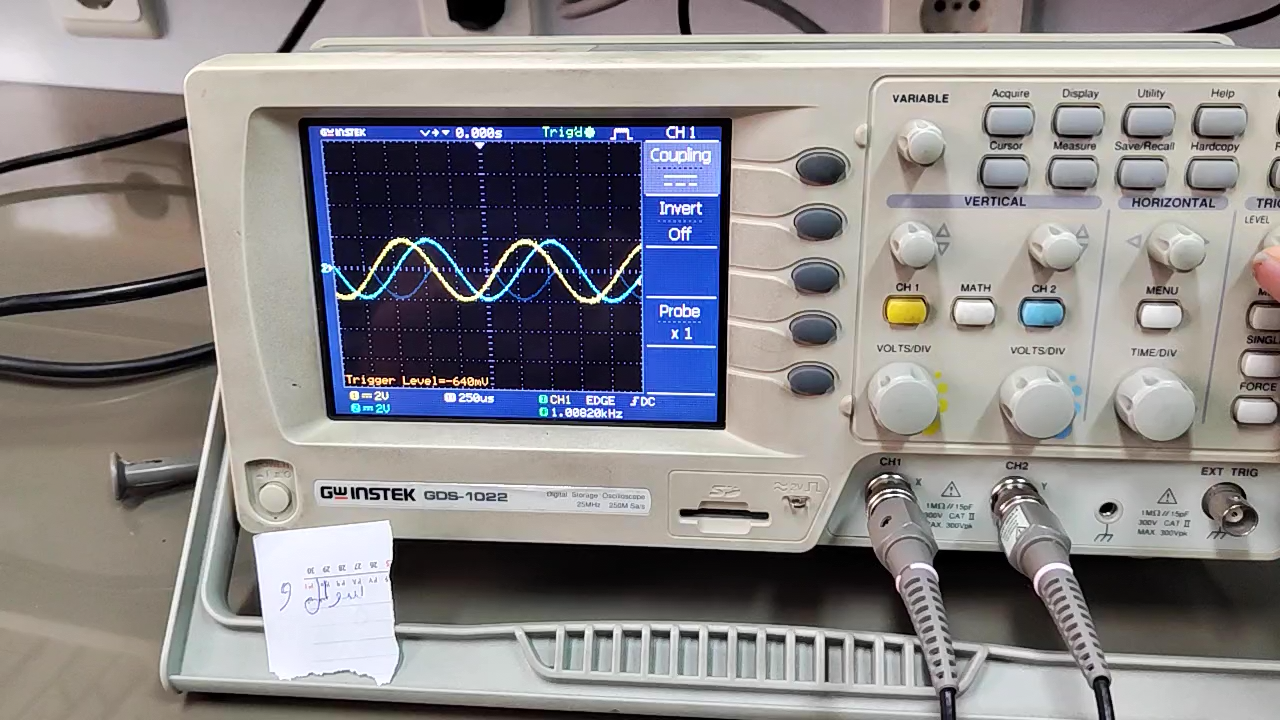
\includegraphics[scale=\PicScale]{Fig/23.png}
                \caption{Two $1$ KHz sine waves produced from two different function generators.}
            \end{center}
        \end{figure}

        \begin{figure}[H]
            \begin{center}
                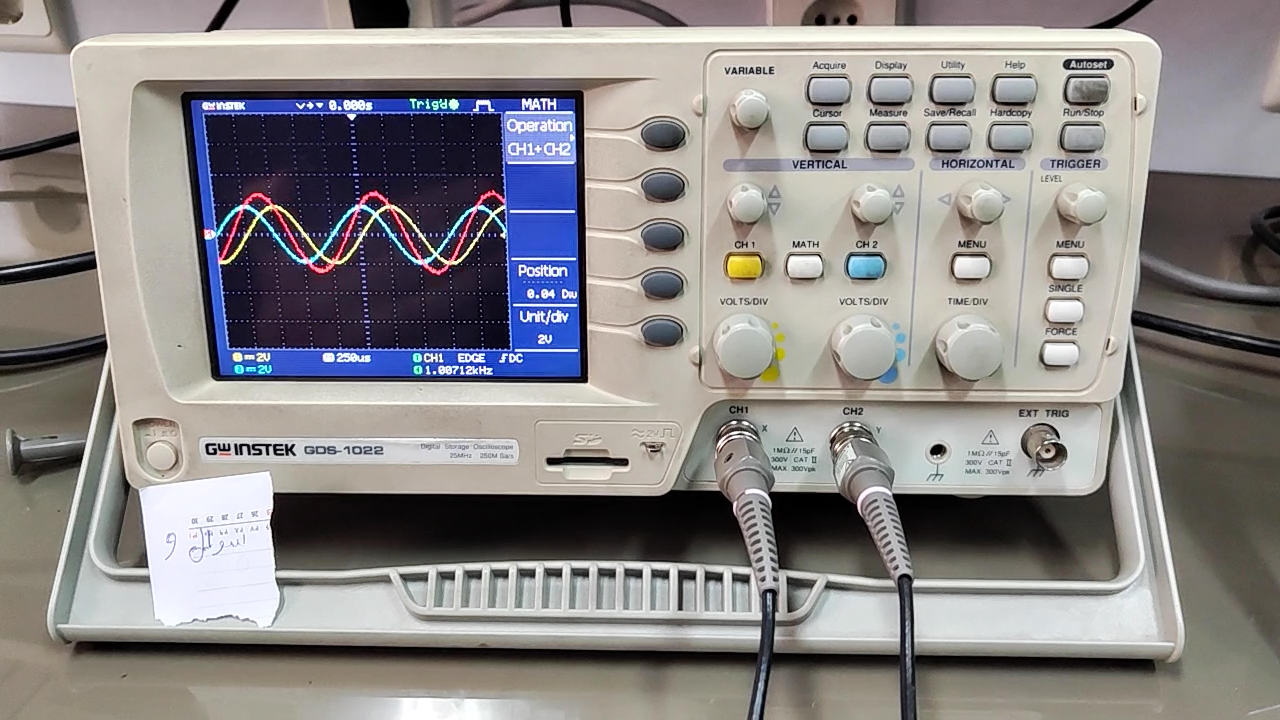
\includegraphics[scale=\PicScale]{Fig/24.png}
                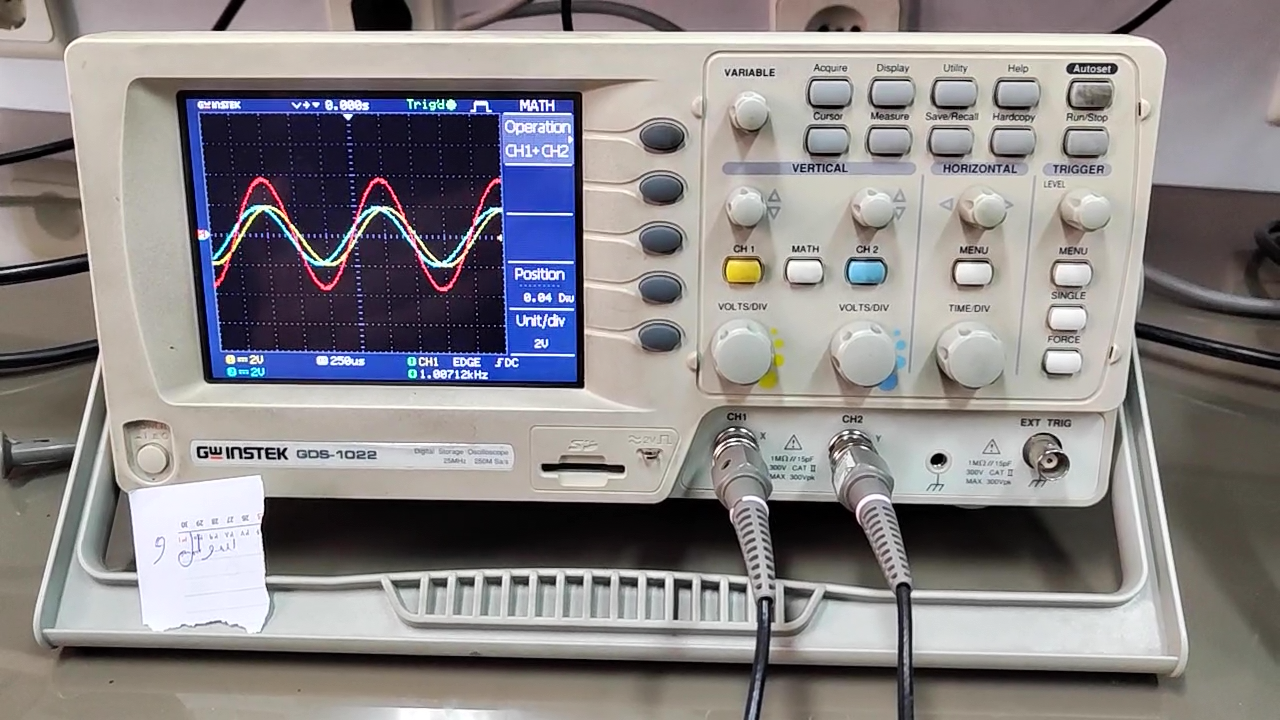
\includegraphics[scale=\PicScale]{Fig/25.png}
                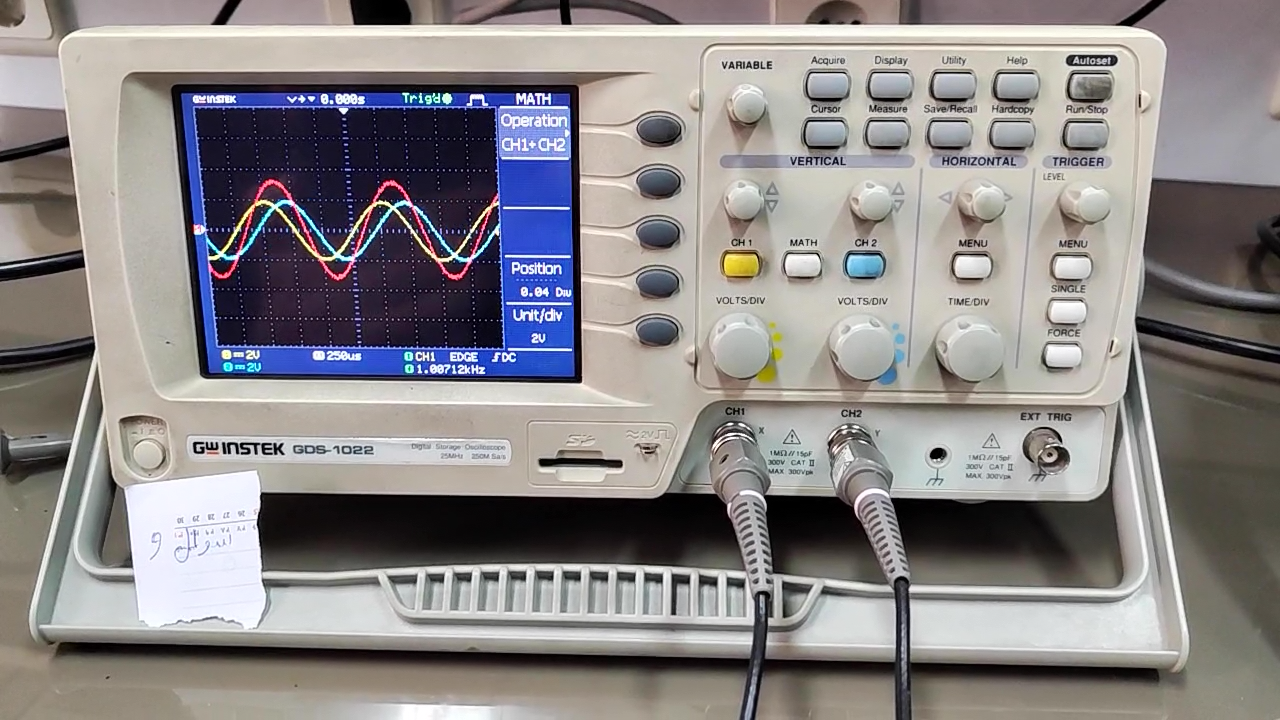
\includegraphics[scale=\PicScale]{Fig/26.png}
                \caption{Two sine waves gathered with each other.}
            \end{center}
        \end{figure}

        \begin{figure}[H]
            \begin{center}
                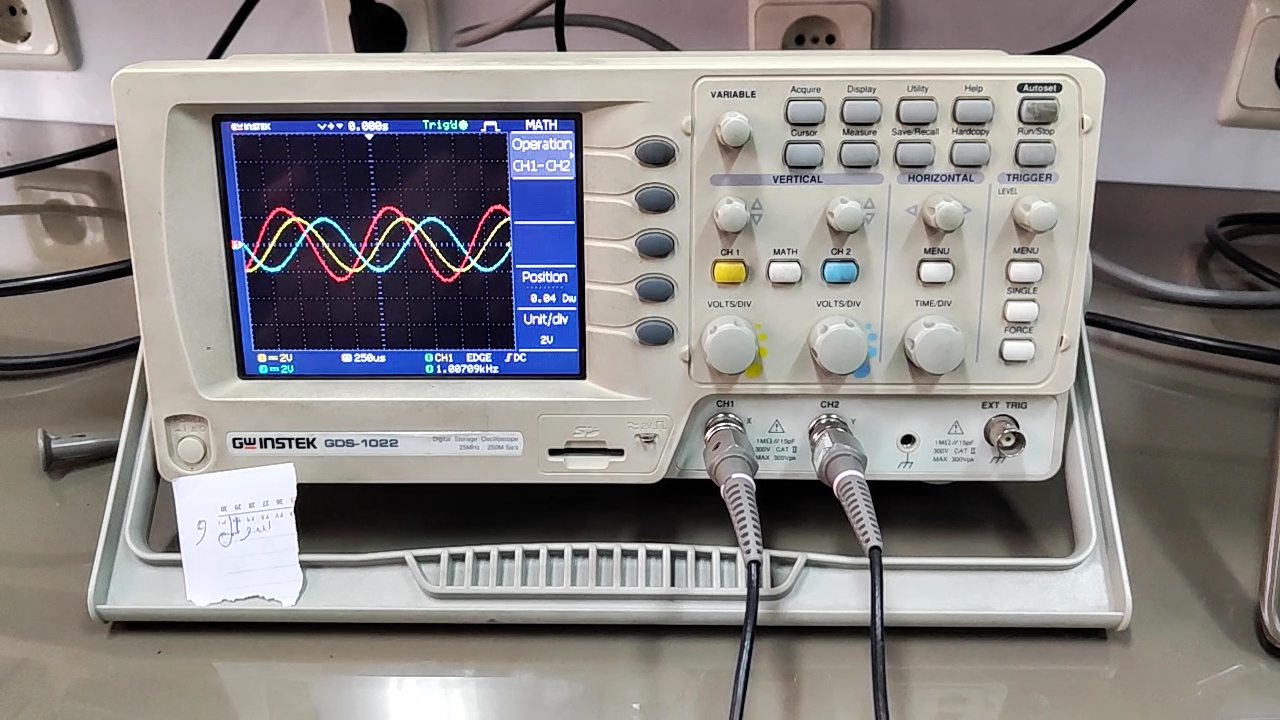
\includegraphics[scale=\PicScale]{Fig/27.png}
                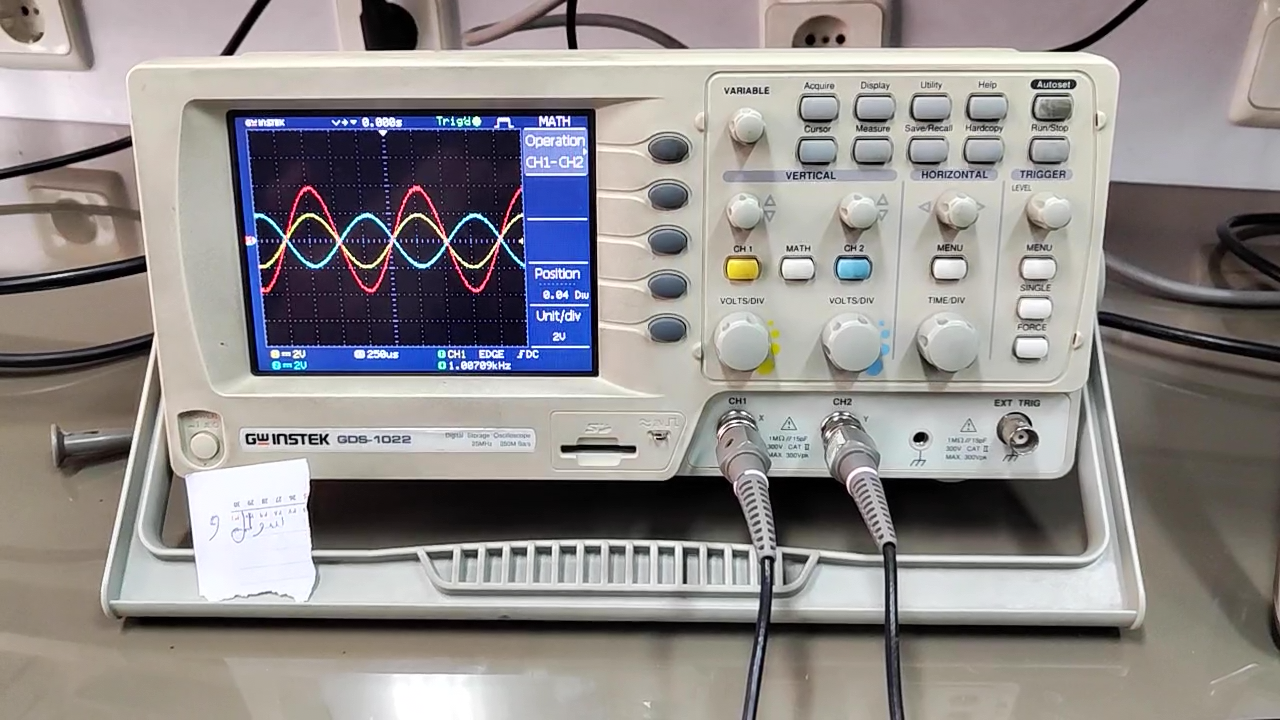
\includegraphics[scale=\PicScale]{Fig/28.png}
                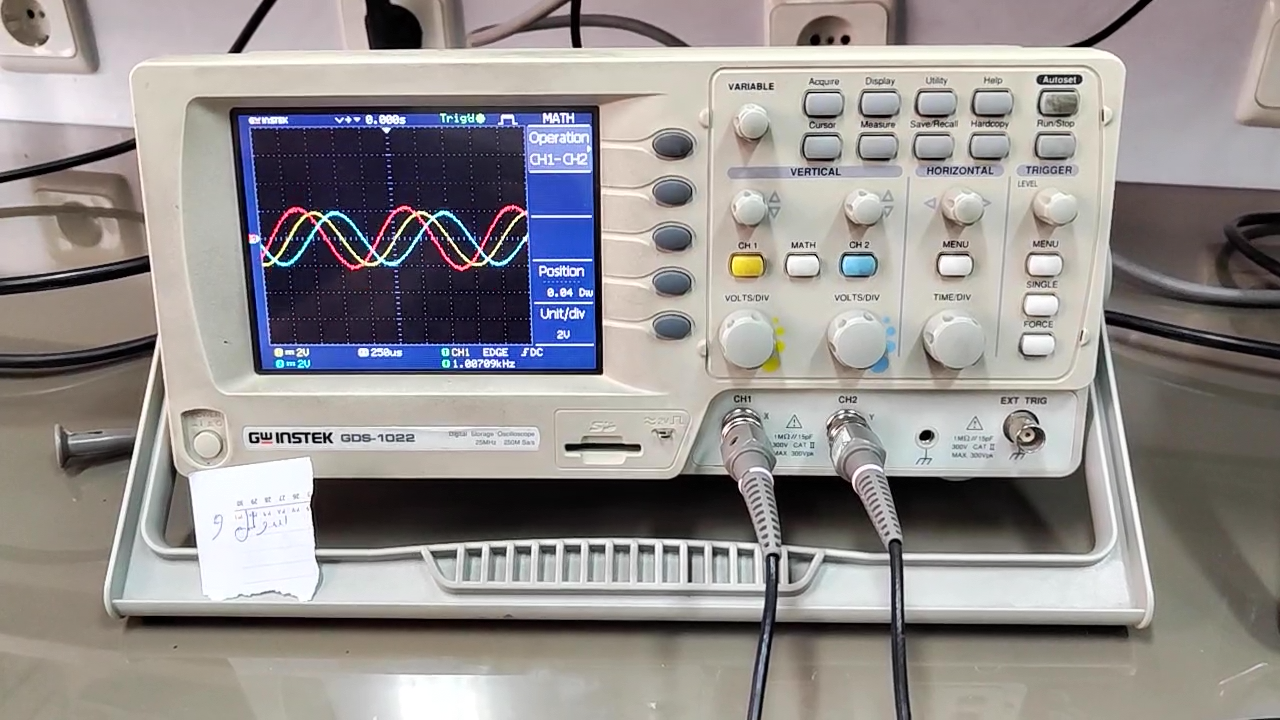
\includegraphics[scale=\PicScale]{Fig/29.png}
                \caption{Two sine waves subtracted from each other.}
            \end{center}
        \end{figure}

    }

\end{question}

%----------------------------------------------------------------------------------------
%	QUESTION 10
%----------------------------------------------------------------------------------------

\begin{question}

    \questiontext{Use the oscilloscope to watch and measure the potential difference between nodes A and B in the circuit of Fig. \ref{fig:cir1}, where the sinusoidal source has a frequency of $1$ kHz and a peak to peak amplitude of $5$ V. Can you measure the desired voltage simply using a single probe? If no, describe the problem and propose a solution.
    }
    \begin{figure}[H]
        \centering
        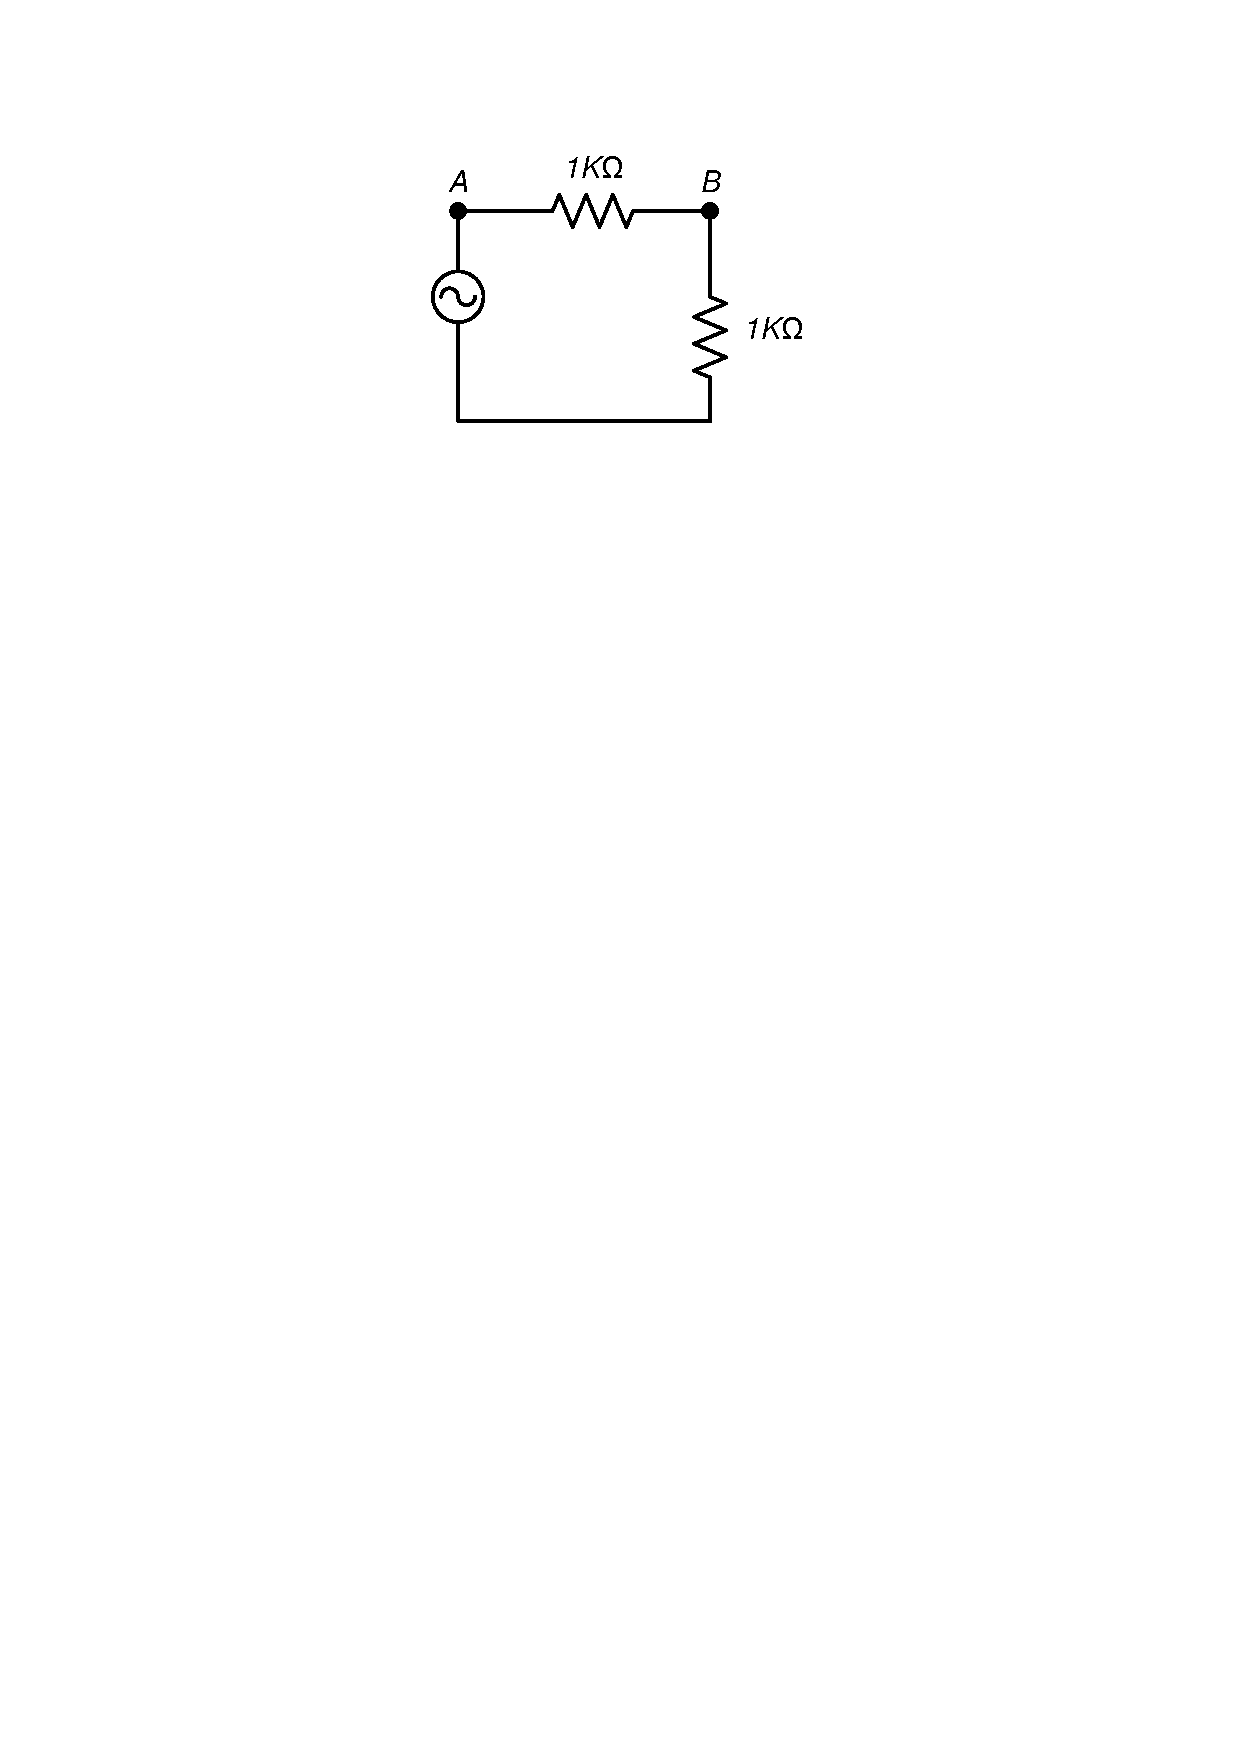
\includegraphics[scale=0.8,angle=0]{Fig/cir1.pdf}
        \caption{A simple resistive circuit.} \label{fig:cir1}
    \end{figure}

    \answer{
        \begin{figure}[H]
            \begin{center}
                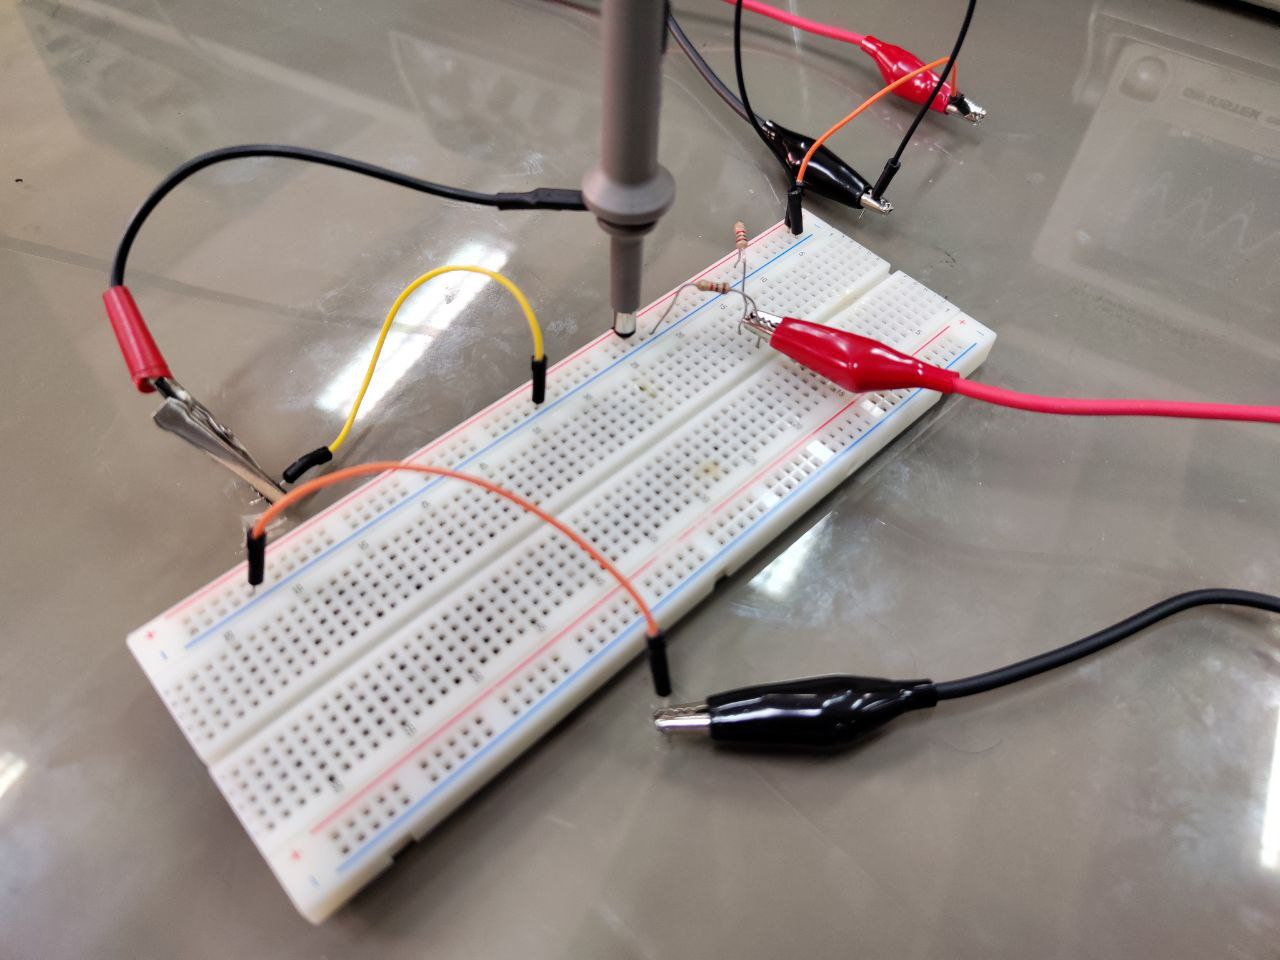
\includegraphics[scale=\PicScale]{Fig/30.jpeg}
                \caption{A simple resistive circuit.}
            \end{center}
        \end{figure}

        \begin{figure}[H]
            \begin{center}
                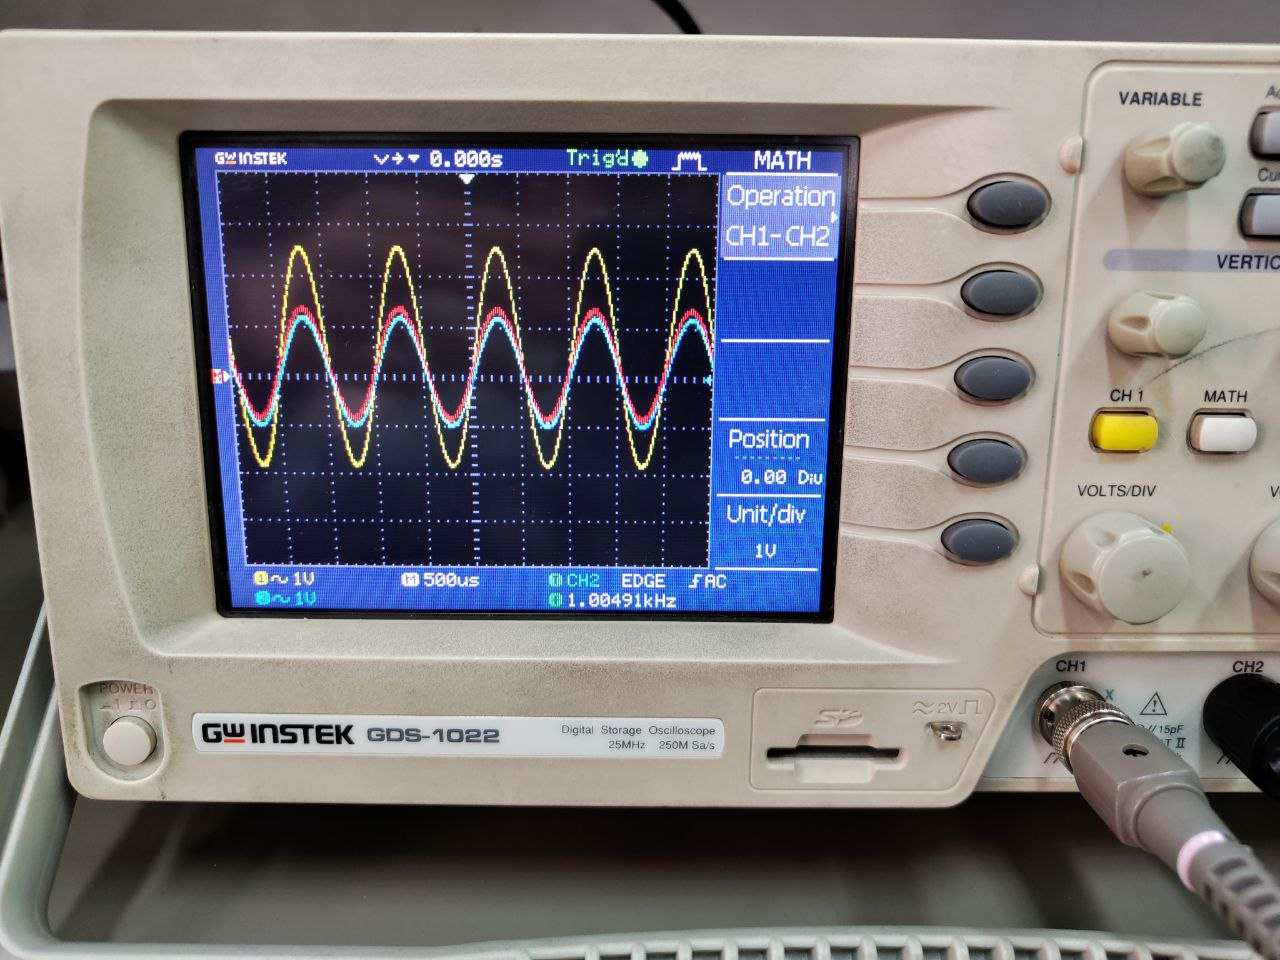
\includegraphics[scale=\PicScale]{Fig/31.jpeg}
                \caption{oscilloscope's picture.}
            \end{center}
        \end{figure}

        \begin{figure}[H]
            \begin{center}
                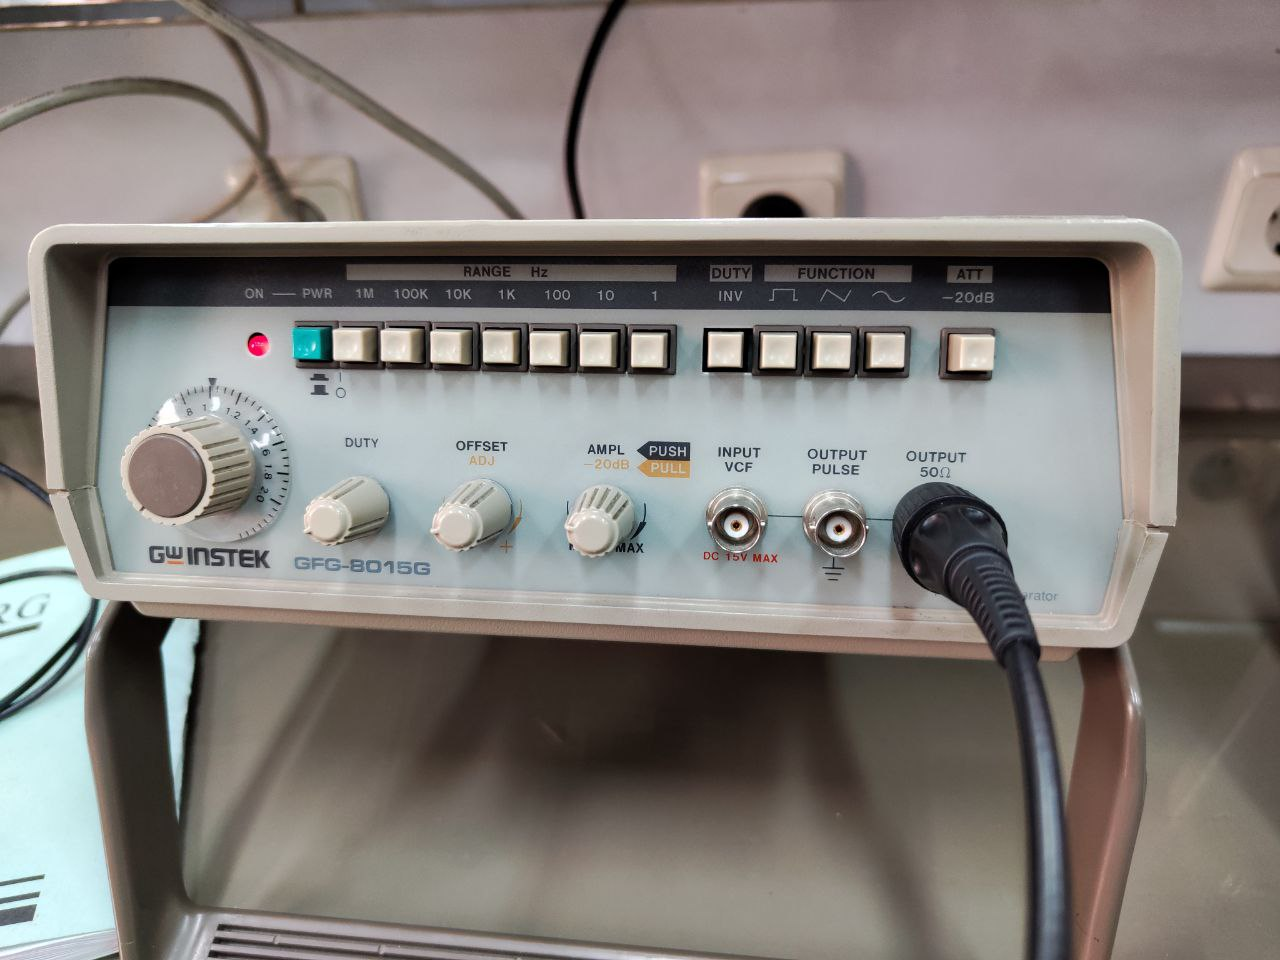
\includegraphics[scale=\PicScale]{Fig/32.jpeg}
                \caption{Function generator's setting.}
            \end{center}
        \end{figure}

        \begin{figure}[H]
            \begin{center}
                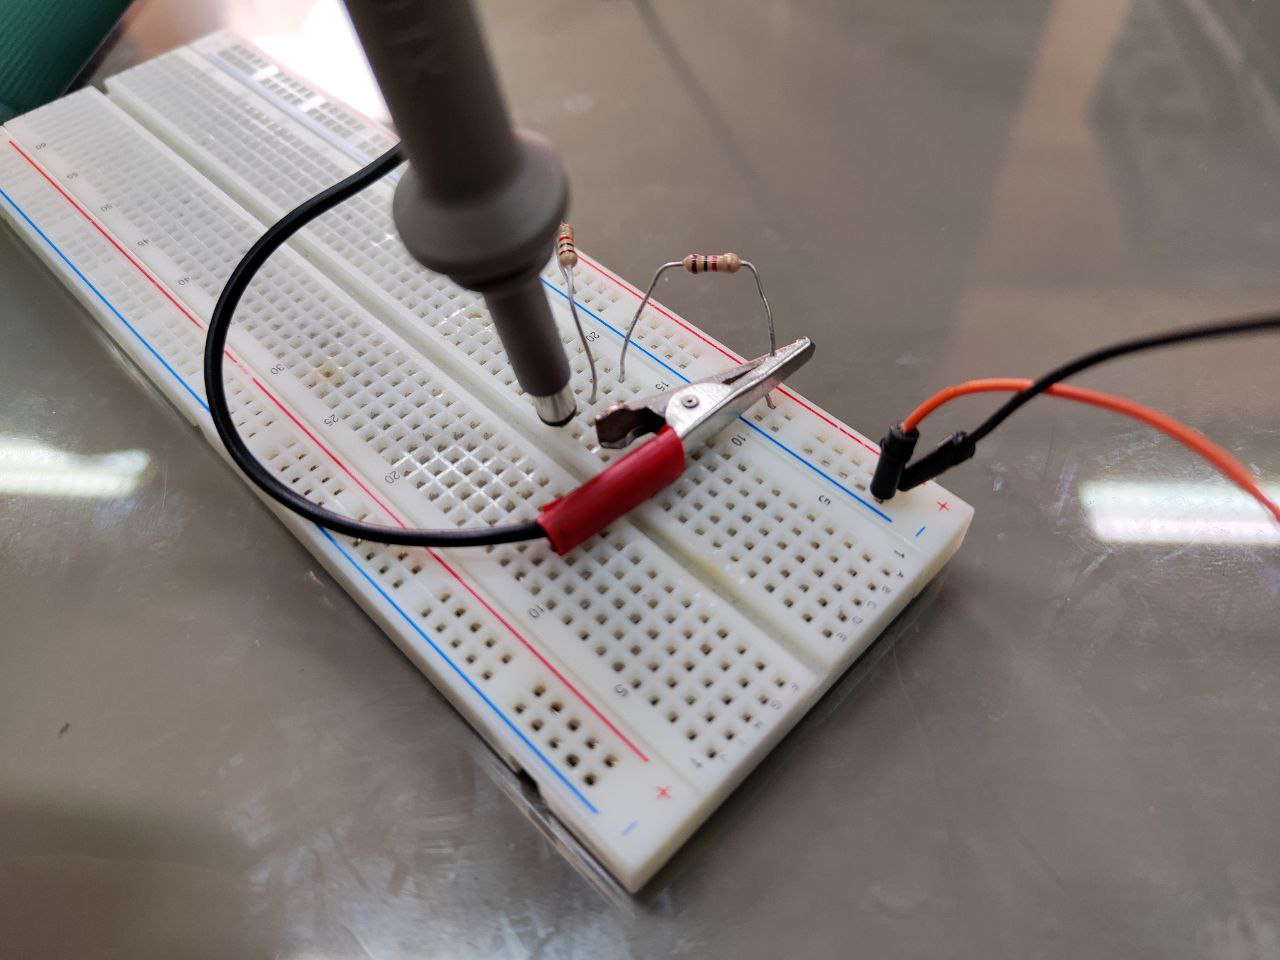
\includegraphics[scale=\PicScale]{Fig/33.jpeg}
                \caption{Circuit related to resistance voltage measurement with a probe.}
            \end{center}
        \end{figure}

        \begin{figure}[H]
            \begin{center}
                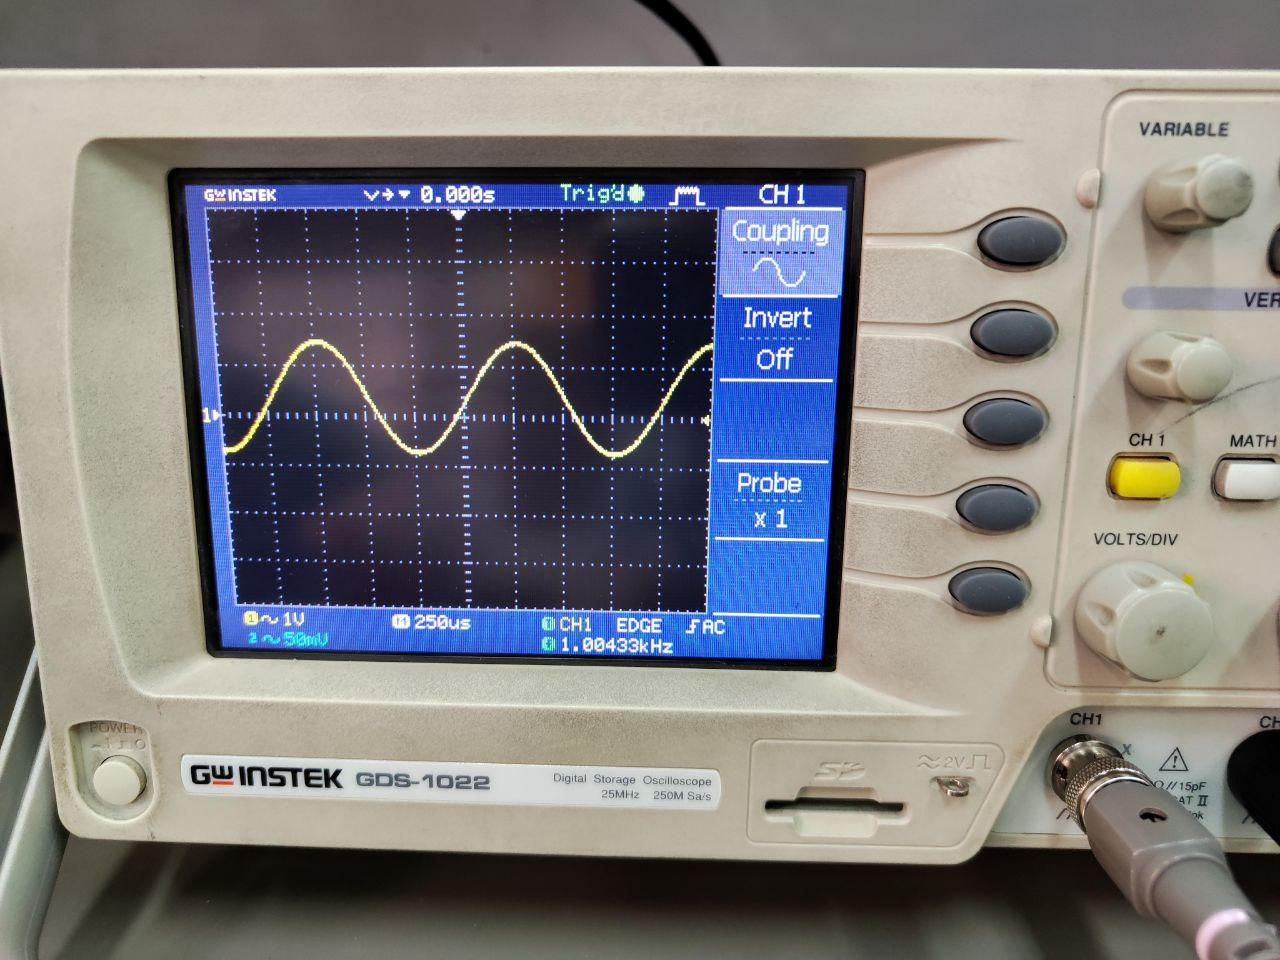
\includegraphics[scale=\PicScale]{Fig/34.jpeg}
                \caption{Measuring resistance voltage with a probe.}
            \end{center}
        \end{figure}
    }

\end{question}

%----------------------------------------------------------------------------------------
%	QUESTION 11
%----------------------------------------------------------------------------------------

\begin{question}

    \questiontext{Set the controls of the function generator to produce a sine wave of $70$ Hz frequency and $1$ V amplitude. Connect the sine wave to the first channel of the oscilloscope and see it for various triggering sources. Discuss the observations.}

    \answer{}

\end{question}

%----------------------------------------------------------------------------------------
%	QUESTION 12
%----------------------------------------------------------------------------------------

\begin{question}

    \questiontext{Change the trigger level and trigger slope in the previous part and analyze your observations.}

    \answer{}


\end{question}

%----------------------------------------------------------------------------------------
%	QUESTION 13
%----------------------------------------------------------------------------------------

\begin{question}

    \questiontext{Feed two sine waves with differences frequencies to two channels of the scope and see the corresponding Lissajous curve on the XY mode. Characterize the Lissajous curve. Is there any relationship between the Lissajous curve and the  frequencies of the sine waves? }

    \answer{}

\end{question}

%----------------------------------------------------------------------------------------
%	QUESTION 14
%----------------------------------------------------------------------------------------

\begin{question}

    \questiontext{Build the circuit of Fig. \ref{fig:cir2} on the breadboard and see the labeled voltages in the XY mode on the oscilloscope screen. Sweep the frequency and amplitudes of the input sine wave and observe the results. Can you interpret the results?
    }
    \begin{figure}[H]
        \centering
        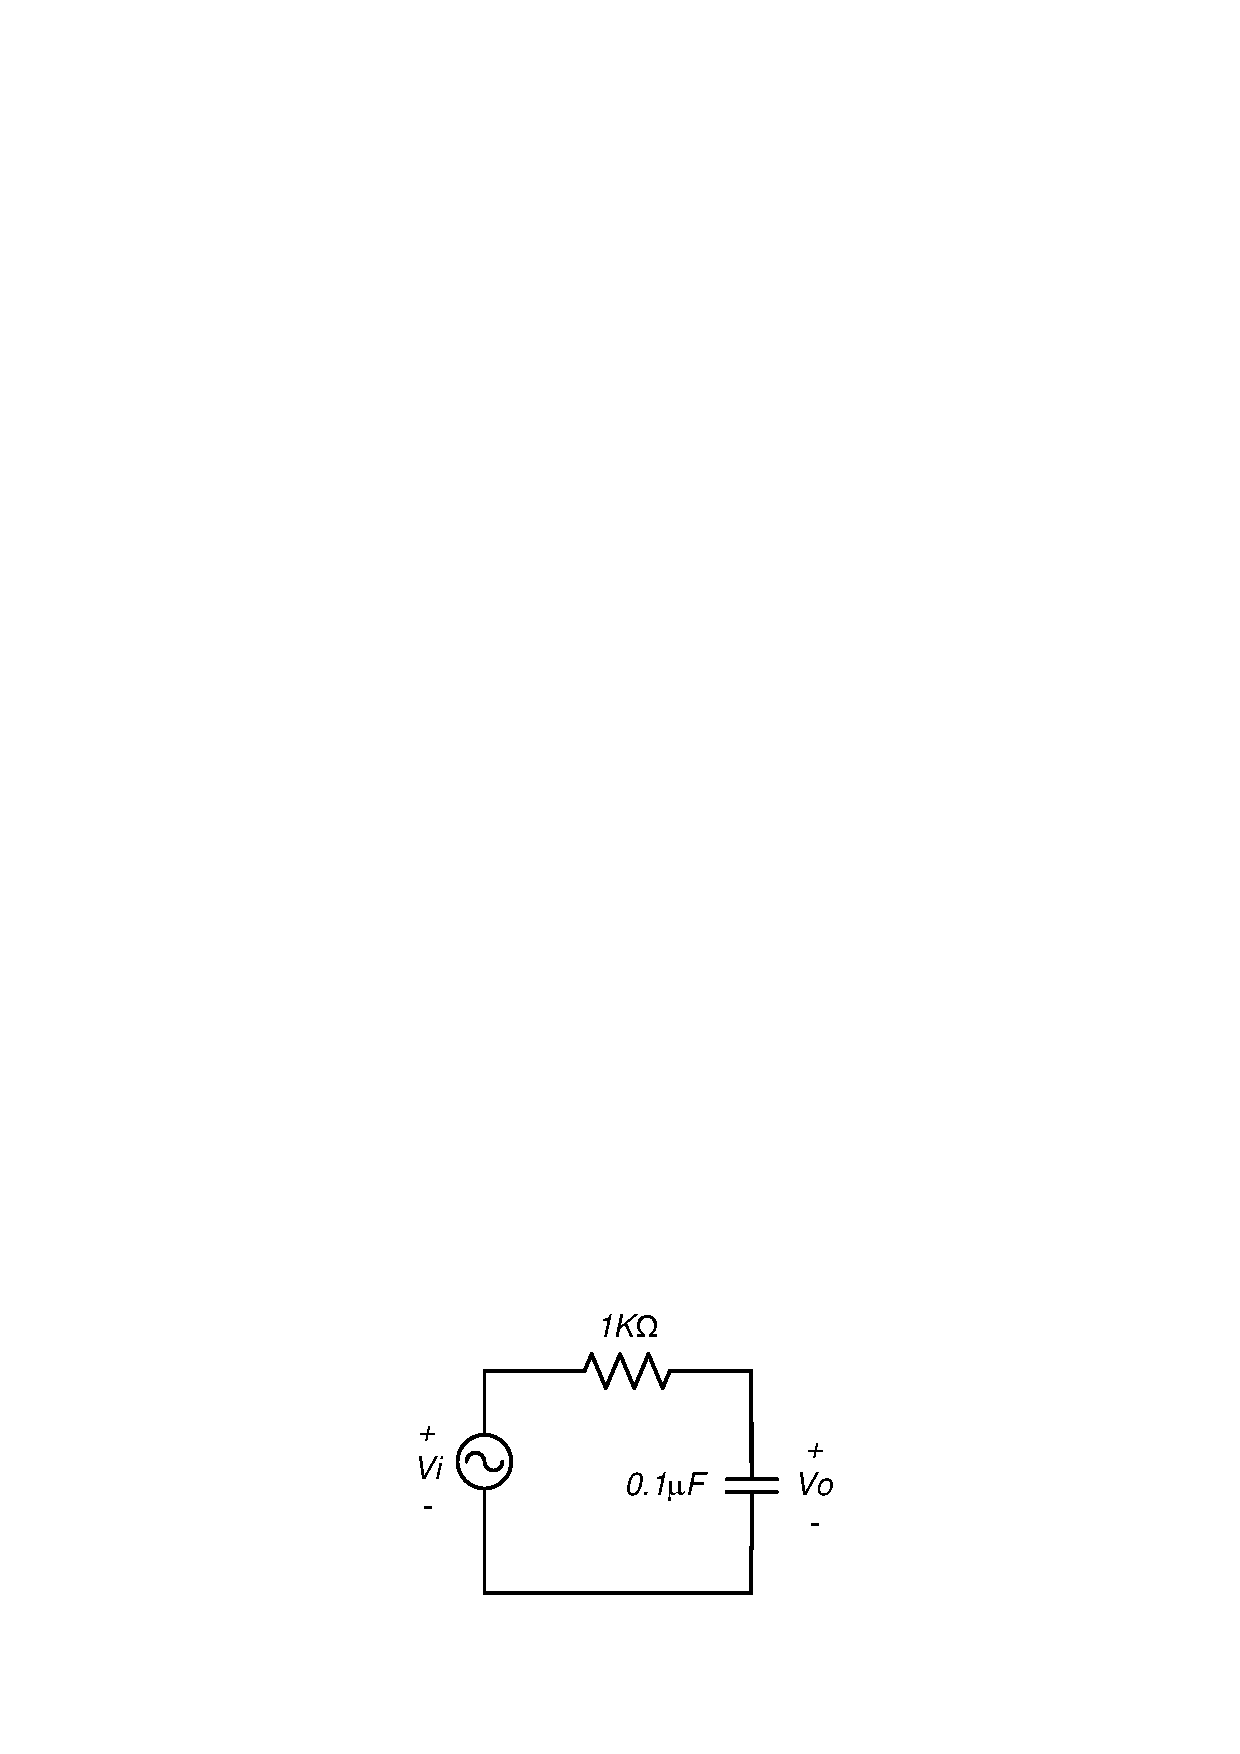
\includegraphics[scale=0.8,angle=0]{Fig/cir2.pdf}
        \caption{An RC circuit.} \label{fig:cir2}
    \end{figure}

\end{question}


\assignmentSection{Bonus Experiments}

%----------------------------------------------------------------------------------------
%	QUESTION 15
%----------------------------------------------------------------------------------------

\begin{question}

    \questiontext{Consider the block diagram of a typical analog oscilloscope shown in Fig. \ref{fig:Q1} and explain how an analog oscilloscope works. How does an analog oscilloscope differ from its digital counterpart? }

    \begin{figure}[H]
        \centering
        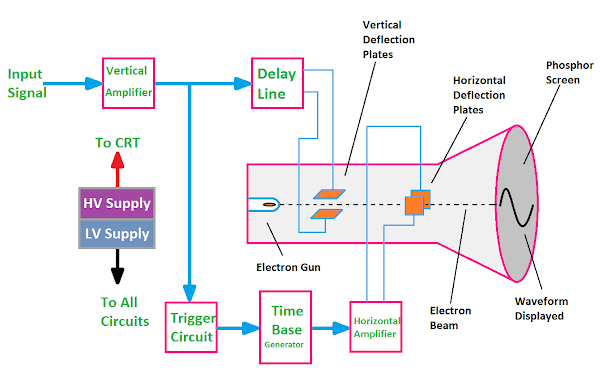
\includegraphics[scale=1,angle=0]{Fig/Q1.png}
        \caption{Block diagram of an analog oscilloscope.} \label{fig:Q1}
    \end{figure}

    \answer{}

\end{question}

%----------------------------------------------------------------------------------------
%	QUESTION 16
%----------------------------------------------------------------------------------------

\begin{question}

    \questiontext{What might lead to a distorted representation of the oscilloscope calibration signal on the screen? What do you offer to resolve the problem?
    }
    \answer{}

\end{question}

%----------------------------------------------------------------------------------------
%	QUESTION 17
%----------------------------------------------------------------------------------------

\begin{question}

    \questiontext{Return your work report by filling the \LaTeX template of the manual. Include useful and high-quality images to make the report more readable and understandable.}

\end{question}

%----------------------------------------------------------------------------------------

\end{document}
